\chapter{Medical Devices: Current State and Challenges}

The medical device market is worth \$289 billion, of which \$110 billion is from the US alone, with this number projected to reach \$133 billion in 2016.
Examples include everything from adhesive bandages, stents, artificial joints, drug infusion pumps to surgical robots, implantable cardiac pacemakers, and devices still undergoing basic research like the artificial pancreas.
To take one example of the societal impact of medical devices, an estimated 3 million people worldwide have implanted cardiac pacemakers (a heart rate adjustment device), with 600,000 added annually.
Clinical trials have presented evidence that patients implanted with cardiac defibrillators (another heart rate adjustment device) have a mortality rate reduced by up to 31\%.
% MADIT II trial
Implanted cardiac pacemakers and defibrillators have approximately 80,000-100,000 lines of software code which essentially makes all sensing, control and actuation decisions autonomously within the human body, over the 5-7 year device lifetime \footnote{Paul L. Jones. Senior Systems/Software Engineer, Office of Science and Engineering
Laboratories, U. S. FDA. Personal communication, 2010.}. With the increasing complexity of combining hardware and software in a large class of these life-saving technologies, there is an urgent need for approaches to rigorously validate the device and therapy to be safe and efficacious.
\begin{figure}[t]
		\centering
		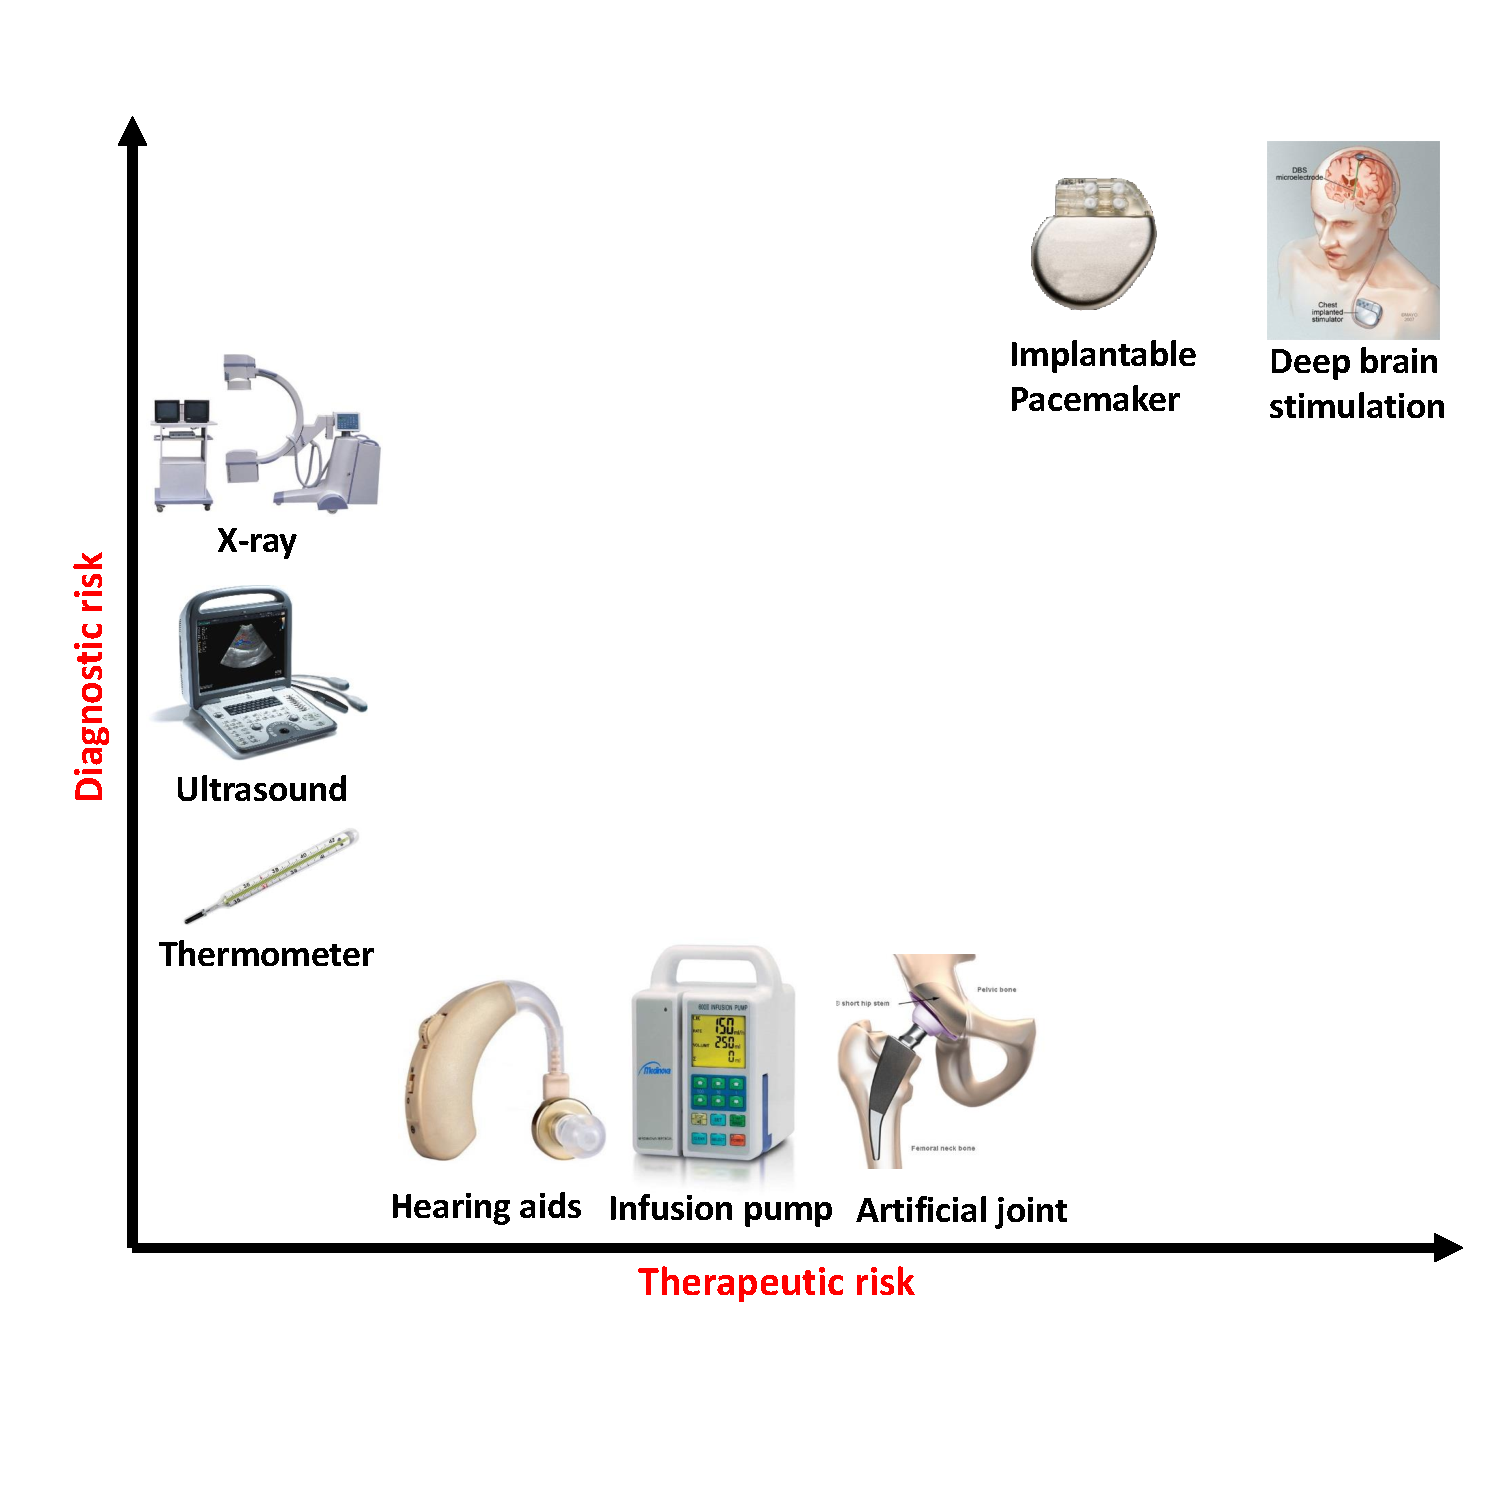
\includegraphics[width=\textwidth]{figs/devices_new.pdf}
		\caption{\small Current medical devices across a range of diagnostic and therapeutic risk. Implantable software-controlled devices such as the pacemaker and defibrillator which operate in a closed-loop of sensing, control and actuation are amongst the highest risk}
		\vspace{-10pt}
		\label{fig:Cur}
\end{figure}

The US Food and Drug Administration defines a medical device as an instrument, apparatus, implement, machine, or implant which is:
\begin{itemize}
	\item intended for use in the diagnosis of disease or other conditions, or in the cure, mitigation, treatment, or prevention of disease, in humans or other animals, or
	\item intended to affect the structure or any function of the human body or other animals, and which does not achieve any of its primary intended purposes through chemical action and which is not dependent upon being metabolized for the achievement of any of its primary intended purposes."
\end{itemize}
\newpage
In general, medical devices are categorized according to their risk factors - Class I, Class II and Class III, corresponding to low-risk, medium-risk and high-risk devices (\cite{class}).  \figref{Cur} gives an intuitive description of medical devices examples across a range of diagnostic and therapeutic risk.


%%On similar lines, in the European Union there are five medical devices categories based on non-invasive vs. invasive, length of stay in body, contact with blood vessels or the central nervous system, active vs. non-active and implantable devices. (\cite{EU_classify}) 
%%Invasive devices with active interventions are subject to stringent regulations to ensure the patient's safety and efficacy of therapy.
\begin{figure}[t]
		\centering
		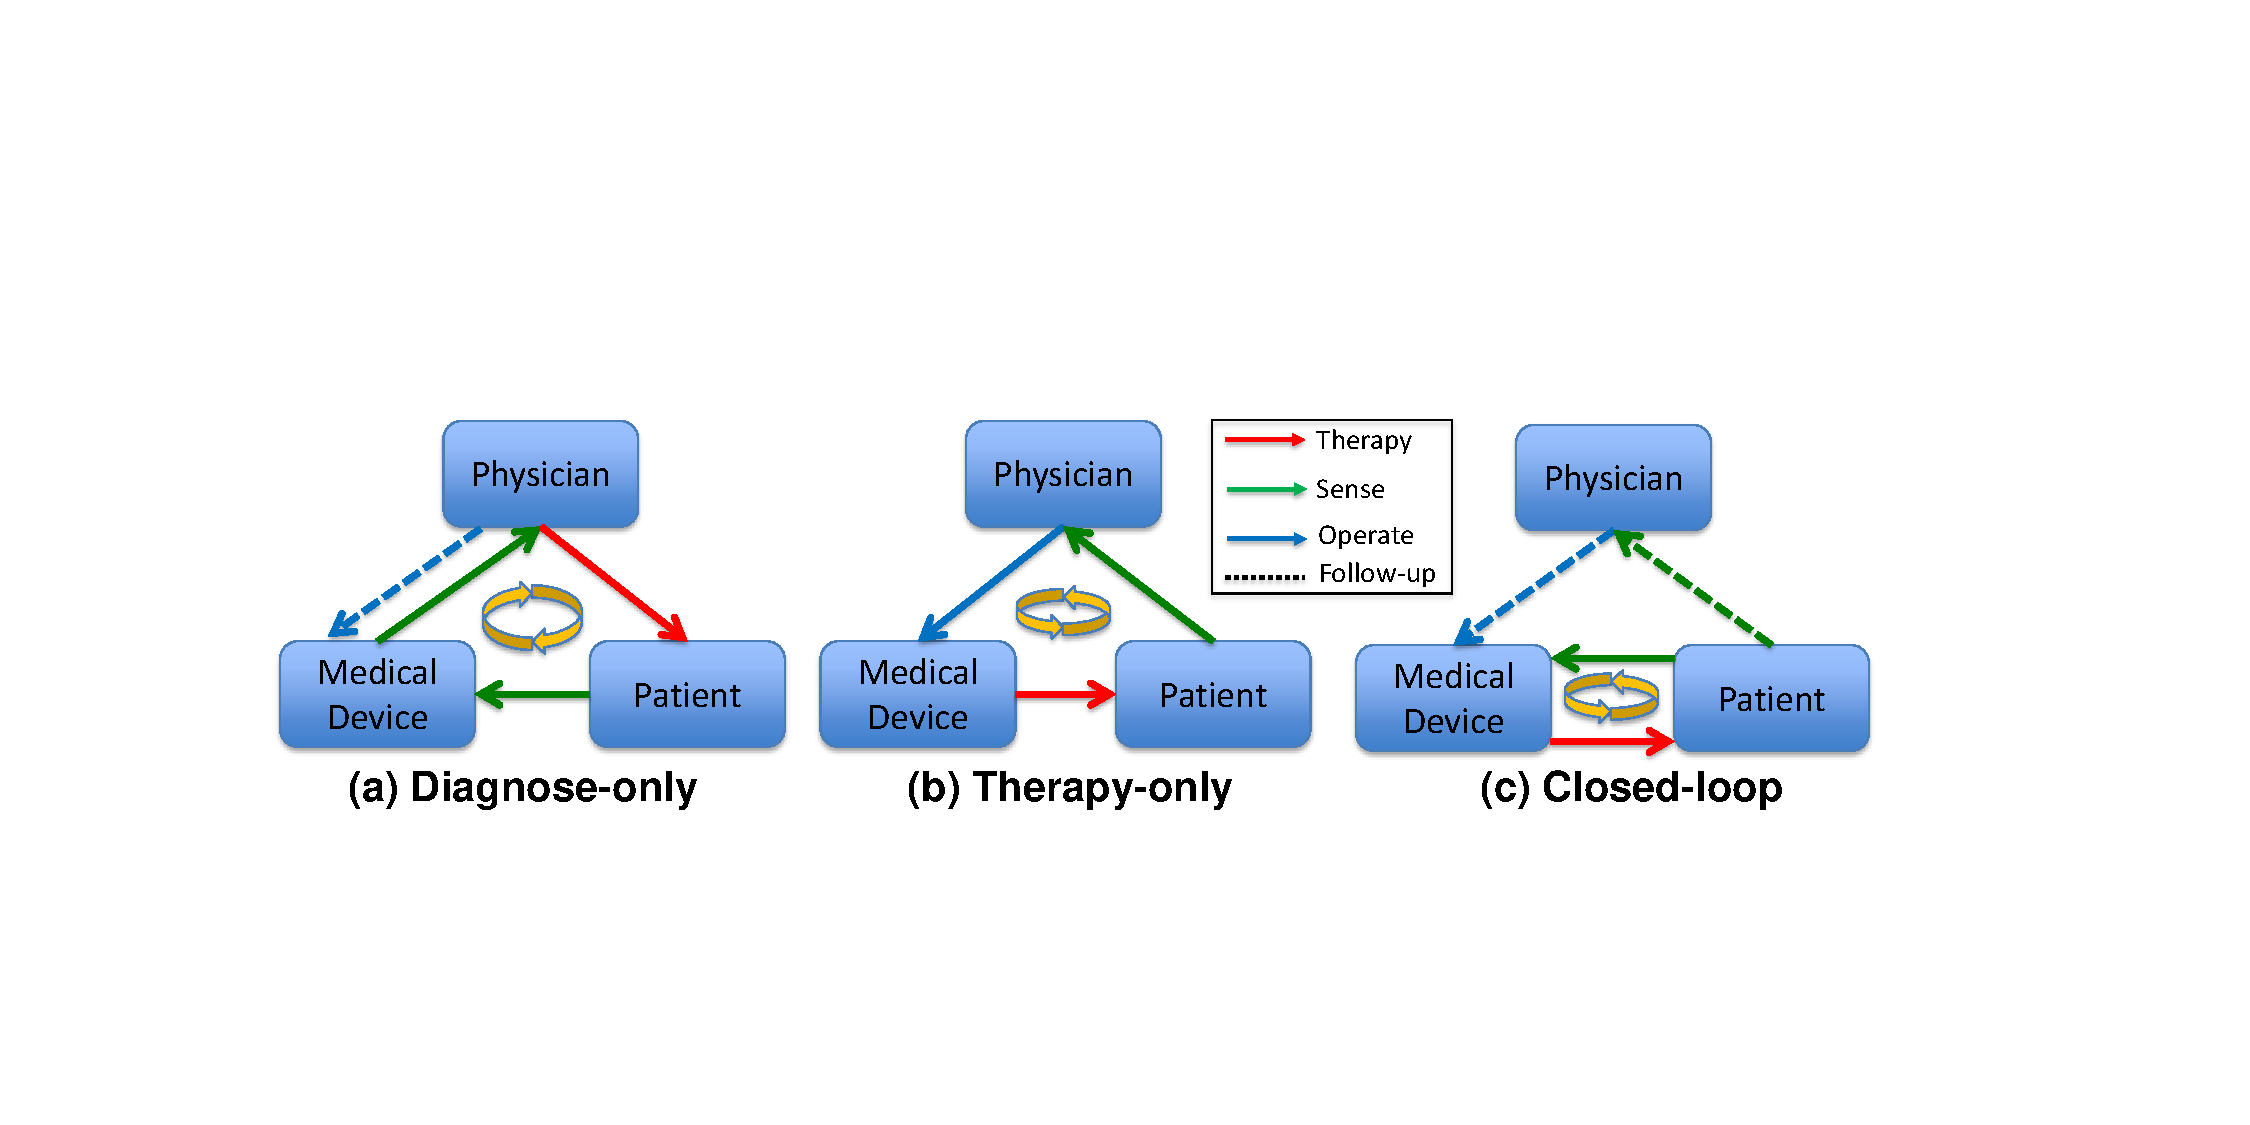
\includegraphics[width=\textwidth]{figs/closed-loop.pdf}
		\caption{\small Diagnostic-only and therapy-only devices do not interact with the patient in direct closed-loop. The physician is responsible for the diagnostic and/or therapeutic decisions. However in closed-loop medical devices, the devices interact with the patient in closed-loop and have to make therapeutic decisions based on their own diagnosis.}
		\label{fig:closed-loop}
\end{figure}
\section{Closing the Device-Patient Loop}
Medical devices operate across a range of invasiveness and intervention with the patient in the loop. For diagnostic-only devices, like an X-ray machine, the physician operates the device to obtain patient data. Upon interpretation of the data, the physician performs diagnosis followed by delivery of proper therapy to the patient (\figref{closed-loop}.(a)). For therapy-only devices, e.g. a drug infusion pump, the physician configures the device infrequently based on prior diagnosis of the patient so the device executes the therapy on the patient (\figref{closed-loop}.(b)). We denote these devices as \textbf{Open-loop Medical Devices} as there is no direct feedback loop between the patient and the device. For open-loop devices, the device operates under the supervision of professionally-trained physicians. The device's safety is mostly determined by how accurately it provides information to the physicians or how faithfully it operates as instructed by the physicians.

There is a class of devices with both diagnostic and therapeutic functions, i.e. implantable cardiac devices to treat cardiac arrhythmia, deep brain stimulation devices (\cite{Brain_sti}) to treat Parkinson's disease and artificial pancreas to treat Type-1 diabetes. These devices capture and diagnose the patient's physiological conditions from sensory data, \emph{and} deliver therapy in response (\figref{closed-loop}.(c)). These devices usually operate (semi-) autonomously with very little human intervention. 
The benefits of closed-loop medical devices are timely therapy and better life-style.
However, autonomy of these medical devices also arose safety concerns. 
Malfunctions or inappropriate therapies from these devices also cannot be corrected timely, which can cause serious adverse effects on patients' health. 
With open-loop medical devices, the diagnosis and therapy decisions are made by medical professionals, who have expert knowledge of human physiology. Therefore they are able to identify adverse health conditions and adjust the therapy accordingly. On the other hand, closed-loop medical devices have to make both the diagnosis and therapy decisions on their own. The domain expertise required to make those decisions has to be programmed into the device. It is impossible to encode all the knowledge of human physiology into the device. Therefore, for unanticipated physiological conditions, when the appropriate response has not been programmed into the device, the device may deliver inappropriate therapy which can have an adverse effect on patient's health. 
Therefore, these devices are usually classified into the highest risk category and undergo the most stringent regulation. We denote them as \textbf{Closed-loop Medical Devices}. 

There are multiple challenges to develop safe and effective closed-loop medical devices:

\subsection{Closed-loop Interactions with Complex Physiology}


Technological development of materials, sensors, embedded computing, energy storage, communications and packaging usher new closed-loop therapies (e.g. deep brain stimulation). While the spectrum of closed-loop interactions between the device and the human physiology may not be fully understood, the challenge is to ensure the device never drives the patient into an adverse state under all physiological conditions. Furthermore, the incremental addition of new therapies in legacy devices (e.g. cardiac rhythm therapy), may result in conflicted diagnostics and behavior of the device for well-understood behaviors and result in inappropriate and unsafe operations. 

\subsection{Limited Diagnostic and Therapeutic Functions}
One fundamental rationale behind closed-loop medical devices is to enable patients to live their  lives normally with limited explicit interaction with the device, and also with minimal physician supervision. In fact, a large number of closed-loop medical devices are autonomous implantable devices. As a result, the sensing and therapy capabilities of these devices are limited, in order to minimize power consumption, heat dissipation and invasiveness. Limited sensing capabilities, and hence limited observability, may cause misdiagnosis as the device may be unable to distinguish the source between two sensed signals from different conditions that now seem similar and result inappropriate therapy. Due to limited therapeutic capabilities, there exists sub-optimal physiological conditions that are untreatable. The device may even drive the body to a less optimal state by over-treating the patient by preempting the body's natural response. In later chapters, we will describe examples in which an untreatable condition is deteriorated into an adverse condition due to the device interaction.

\subsection{Software-related Medical Device Recalls}
Due to the complexity of the diagnostic and therapeutic functions of the closed-loop devices, these functions are mostly controlled by their software components. 
Software embedded in a medical device, unlike electrical and mechanical components, does not fail due to corrosion, fatigue or have statistical failures of subcomponents. Software failures are uniquely sourced in the design and development of the system. %Unlike other industries such as consumer electronics where product life cycles are measured in months, software engineering for medical devices often spans a decade and must prioritize safety and efficacy over time to market. 
%\begin{figure}[t]
		%\centering
		%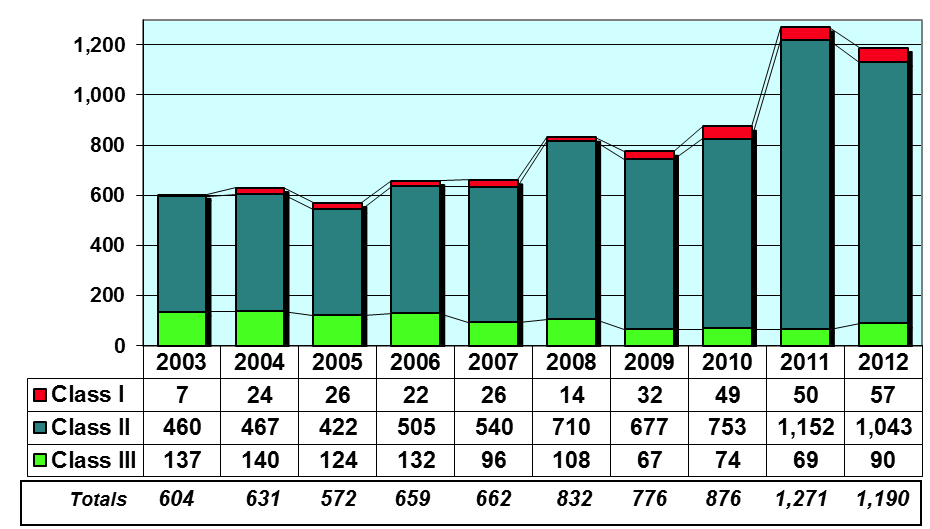
\includegraphics[width=0.8\textwidth]{figs/recalls.jpg}
		%\caption{\small Medical device recalls have risen over the past decade}
		%\label{fig:recalls}
%\end{figure}
\begin{figure}[t]
		\centering
		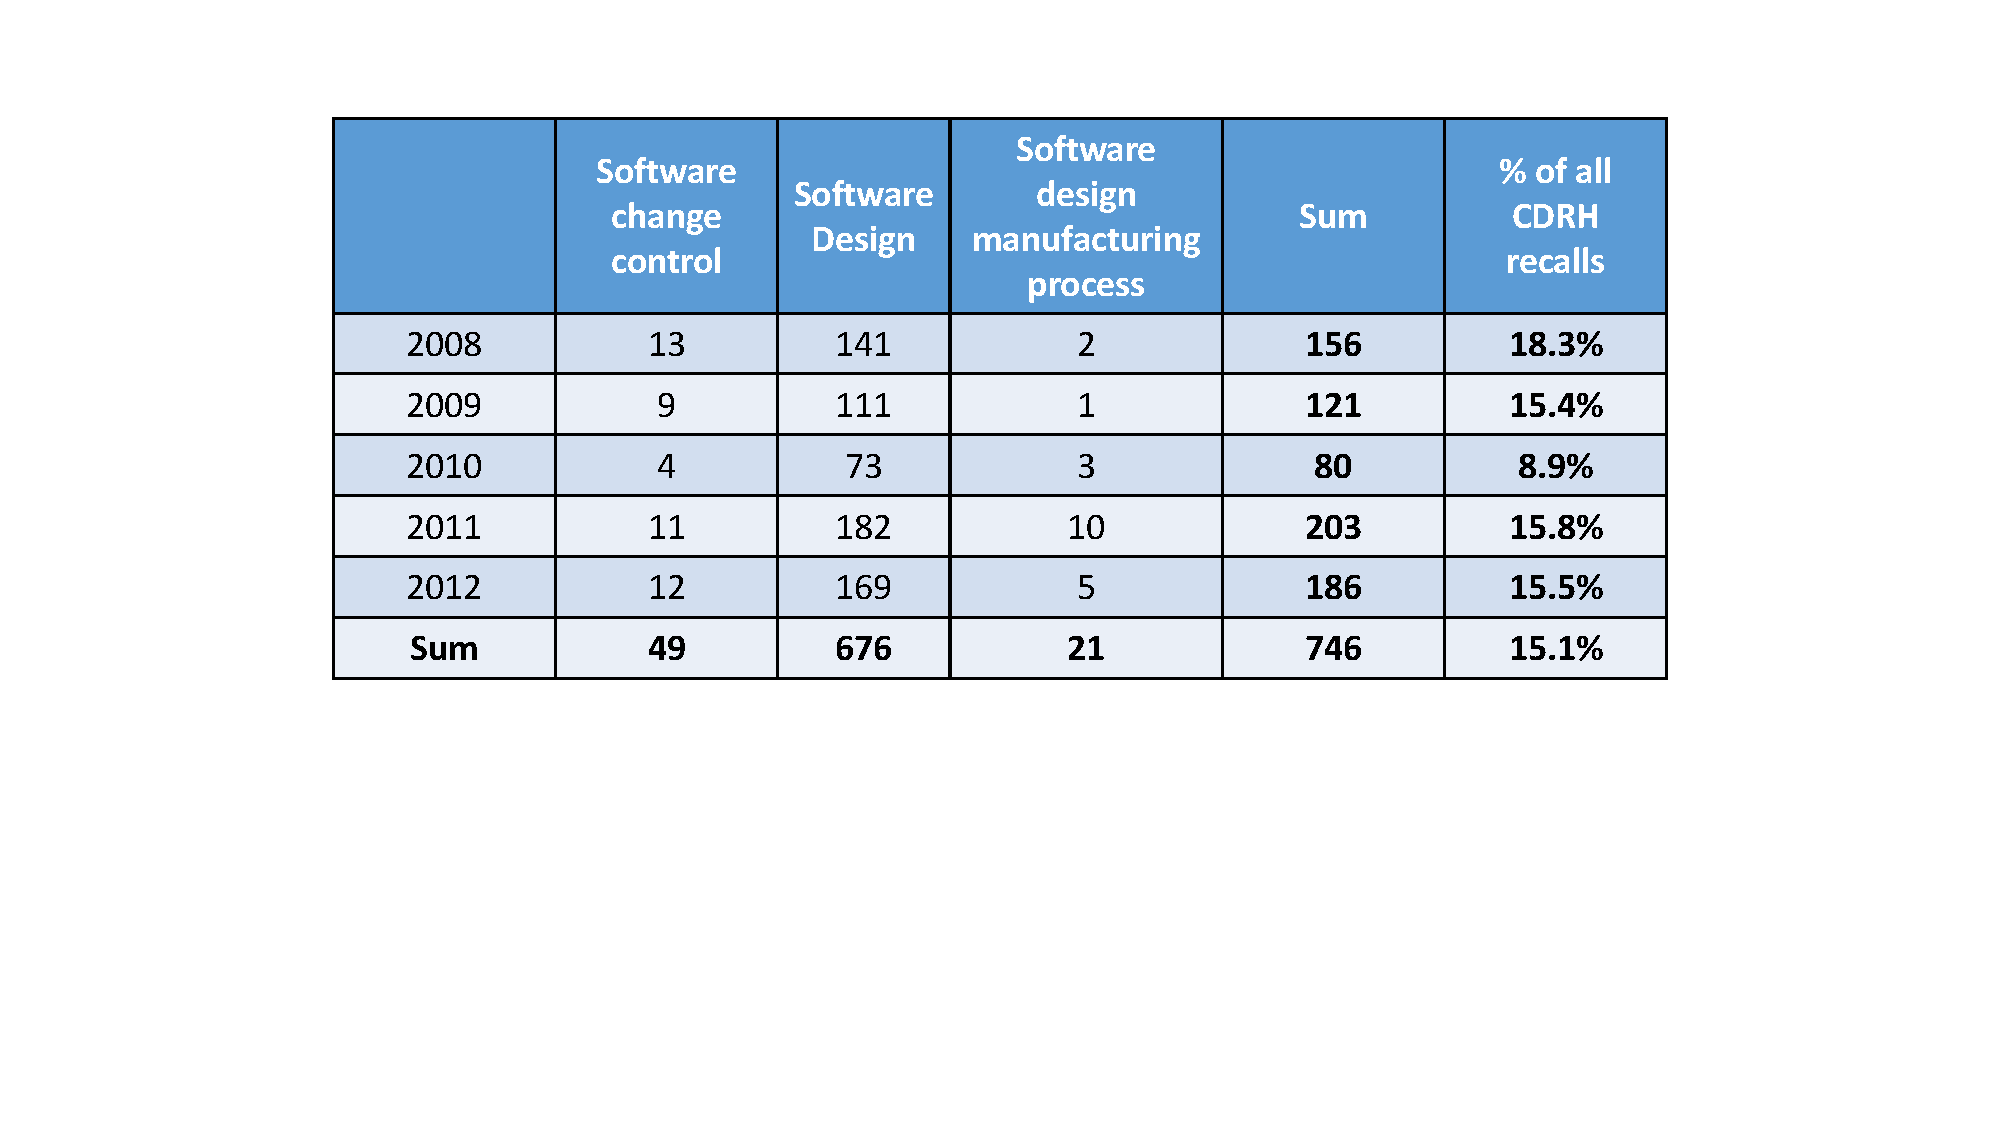
\includegraphics[width=0.8\textwidth]{figs/recalls.pdf}
		\caption{\small Medical device recalls due to software issues have risen from 10\% in the 1990s to \~15\% in the past decade (\cite{recall_rep})}
		\label{fig:soft_recalls}
\end{figure}
%  Over the course of the past four decades, cardiac rhythm management devices such as pacemakers and implantable cardioverter defibrillators (ICD) have grown in complexity and now have more than 80,000 to 100,000 lines of code (\cite{pauljones}). 
According to the US Food and Drug Administration, in 1996, 10\% of all medical device recalls were caused by software-related issues (\cite{medstats}). This percentage rose to an average of 15\% of recalls from 2008 to 2012 (\figref{soft_recalls}). Malfunctions of closed-loop medical devices usually have severe consequences, which will be categorized as \emph{Class I}, meaning there is a ``reasonable probability that use of these products will cause serious adverse health consequences or death.'' (\cite{medstats2,pacemakerrecalls,killedbycode}). 
\looseness1
\section{Medical Device Regulation Efforts and Challenges}
The medical device industry is regulated to ensure the safety of the patients and the public. In the United States, the FDA is the primary regulatory authority responsible for assuring the safety, efficacy and security of patients using medical devices. Based on the rationale that 1) manufacturers know their devices better than the regulator, and 2) the variety of medical devices requires a variety of approaches, it is the device manufacturers' responsibility to demonstrate the safety and efficacy of the medical devices. Manufacturers are required to complete a pre-market submission before the devices can be released to the market. The level of requirements for the submission is determined by the safety classification of the devices. A set of general guidelines are recommended by the FDA (\cite{fda1, fda2, fda3}) which list the activities that need to be performed to ensure device safety. 

In safety-critical industries such as automotive electronics, avionics and nuclear systems, international standards are enforced for software system development, evaluation, manufacturing and post-market changes (\cite{autosar,avsi}). This awareness is only beginning to enter the medical device industry as compliance with international standards are "recommended" in the aforementioned guidelines (\cite{formal_fda}) but the burden of their interpretation and enforcement is on the device manufacturer. The basic rationale behind these standards is that: if all the risks/hazards of the device are identified and reasonably mitigated, and the device is developed with rigorous process, the device is \emph{reasonably safe}. 
\begin{figure}[t]
		\centering
		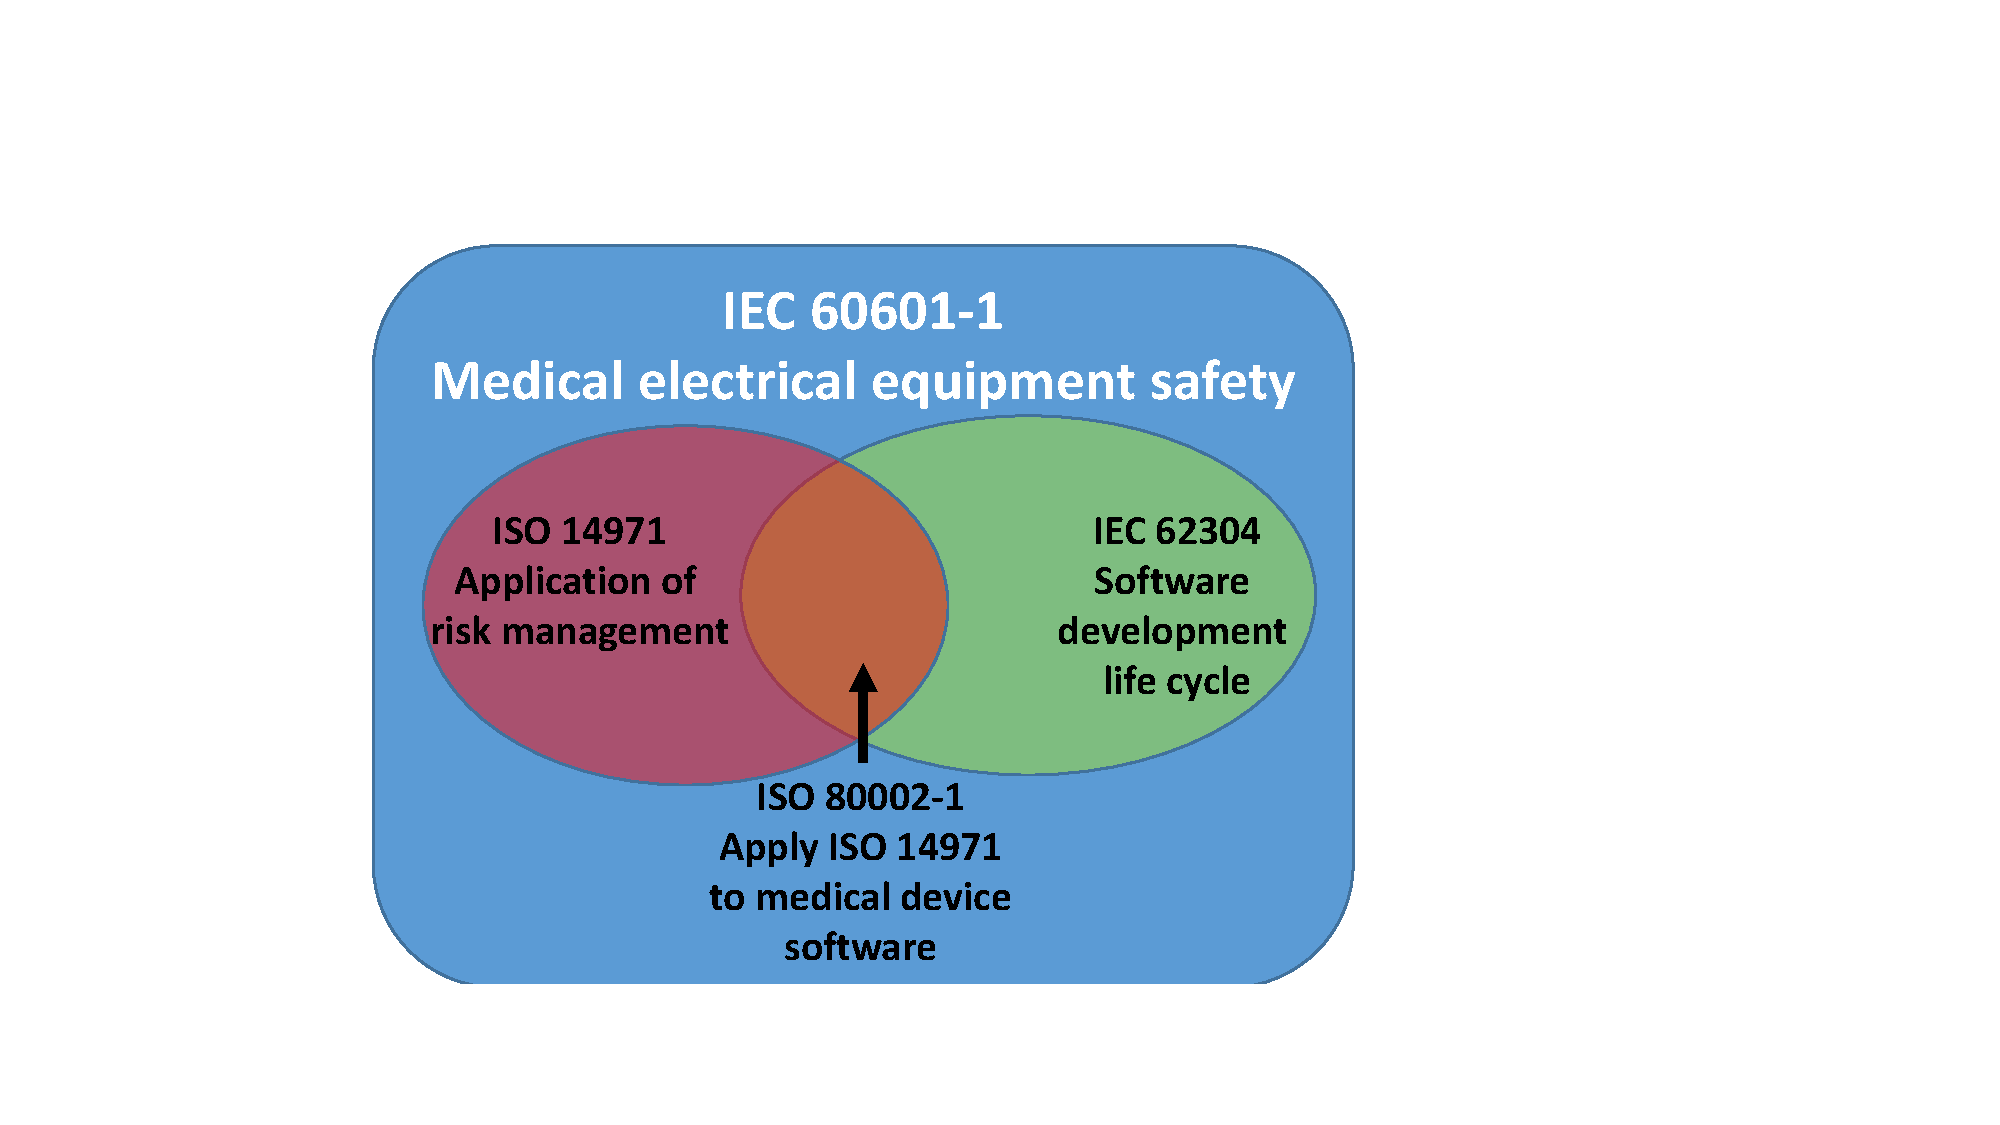
\includegraphics[width=0.6\textwidth]{figs/stardards.pdf}
		\caption{\small International standards for medical device safety. These standards define the required activities during the development process.}
		\label{fig:standards}
\end{figure}

\figref{standards} describes the primary standards to ensure medical device safety and their relationships. The IEC 60601 Medical Electrical Equipment - General requirements for basic safety and essential performance is a product safety standard that all electronic medical devices must comply to. IEC 60324 specifies the processes and activities needed to perform during the software development life cycle to ensure software safety. 

Risk management is a core activity throughout the software development life cycle. ISO 14971 is specified for the application of risk management to medical devices. In addition, for each risk management activity of ISO 14971, ISO 80002-1 provides additional guidelines for the software component, which highlights and explains approaches to assuring that software safety is adequately addressed.

%While the above standards and several others provide guidelines to ensuring software safety they do so in an informal or ad hoc manner with a focus on the rigorousness of the design process rather than on quantitative evaluation on the closed-loop system with the physiological system (or a model) and the feedback to and from the device. Furthermore, there is a separation of concerns where the \emph{regulatory perspective} is on the overall safety of the device meeting its diagnostic and therapeutic requirements within its environment (e.g. pacemaker inside the body and connected with the heart tissue), the \emph{software standards' perspective} is on the device meeting its specifications (e.g. if the pacemaker does not sense an event within a certain interval, then pace the heart). While the device may respond appropriately to the sensed input, we also need to establish that the device never drives the patient to an adverse condition. As the regulatory perspective requires closed-loop safety and the device software's specifications are largely evaluated with open-loop ``tape tests" of pre-recorded signals, with no physiological interaction, this introduces a safety gap.  So a device may meet its software specifications but that does not necessarily ensure it meets the physiological safety requirements. 


%The history of the FDA is a reactionary one, where each stage of evolution was in response to a major healthcare tragedy. 
\begin{figure}[t]
		\centering
		\includegraphics[width=\textwidth]{figs/fta_new.pdf}
		\caption{\small Fault Tree Analysis (FTA) Examples. (a) FTA for a hazard for a car; (b) FTA for a hazard in implantable pacemaker. The dashed line shows two mechanisms that were not identified during hazard analysis but discovered in post-market studies.}
		\label{fig:risks}
\end{figure}
\subsection{Risk Management Challenges of Closed-loop Systems}
While it is not normally possible to develop a device that is safe with a probability of 100\% under all physiological and operating conditions, approaching the problem along the lines of risk analysis, risk evaluation and risk control helps better address a ``designed-for-safety" mindset. Fault Tree Analysis (FTA) is a common tool in risk analysis in which hazards of the system are first identified and the possible causes of the hazards are analyzed until the initial faults are reached. \figref{risks}.(a) demonstrate an example fault tree for automobile. FTA is very good at showing how resistant a system is to single or multiple initiating faults. It is not good at finding all possible initiating faults since causes are conjectured and analyzed manually. 

In closed-loop medical devices, there may exist interactions between the device and the patient that can cause certain hazard, but are unknown due to limits in physiological knowledge, behavior not captured in patient trials and the separation of the software development teams and the medical domain experts. \figref{risks}.(b) describes an example fault tree for a hazard for an implantable pacemaker. There are several causes for undesirable fast ventricular rate. The well-understood cause is the intrinsic ventricular tachycardia (solid line). However, with pacemaker implanted, new mechanisms to cause hazard are introduced into the closed-loop system, as illustrated by the two branches with dotted lines. These two branches were not identified during the initial fault tree analysis, and were only identified after the devices have been released into the market, causing unnecessary adverse effects to the patients \cite{ELT}. Risks identified at this late stage are also more costly to fix, increasing the cost for device development. 


\begin{figure}[t]
		\centering
		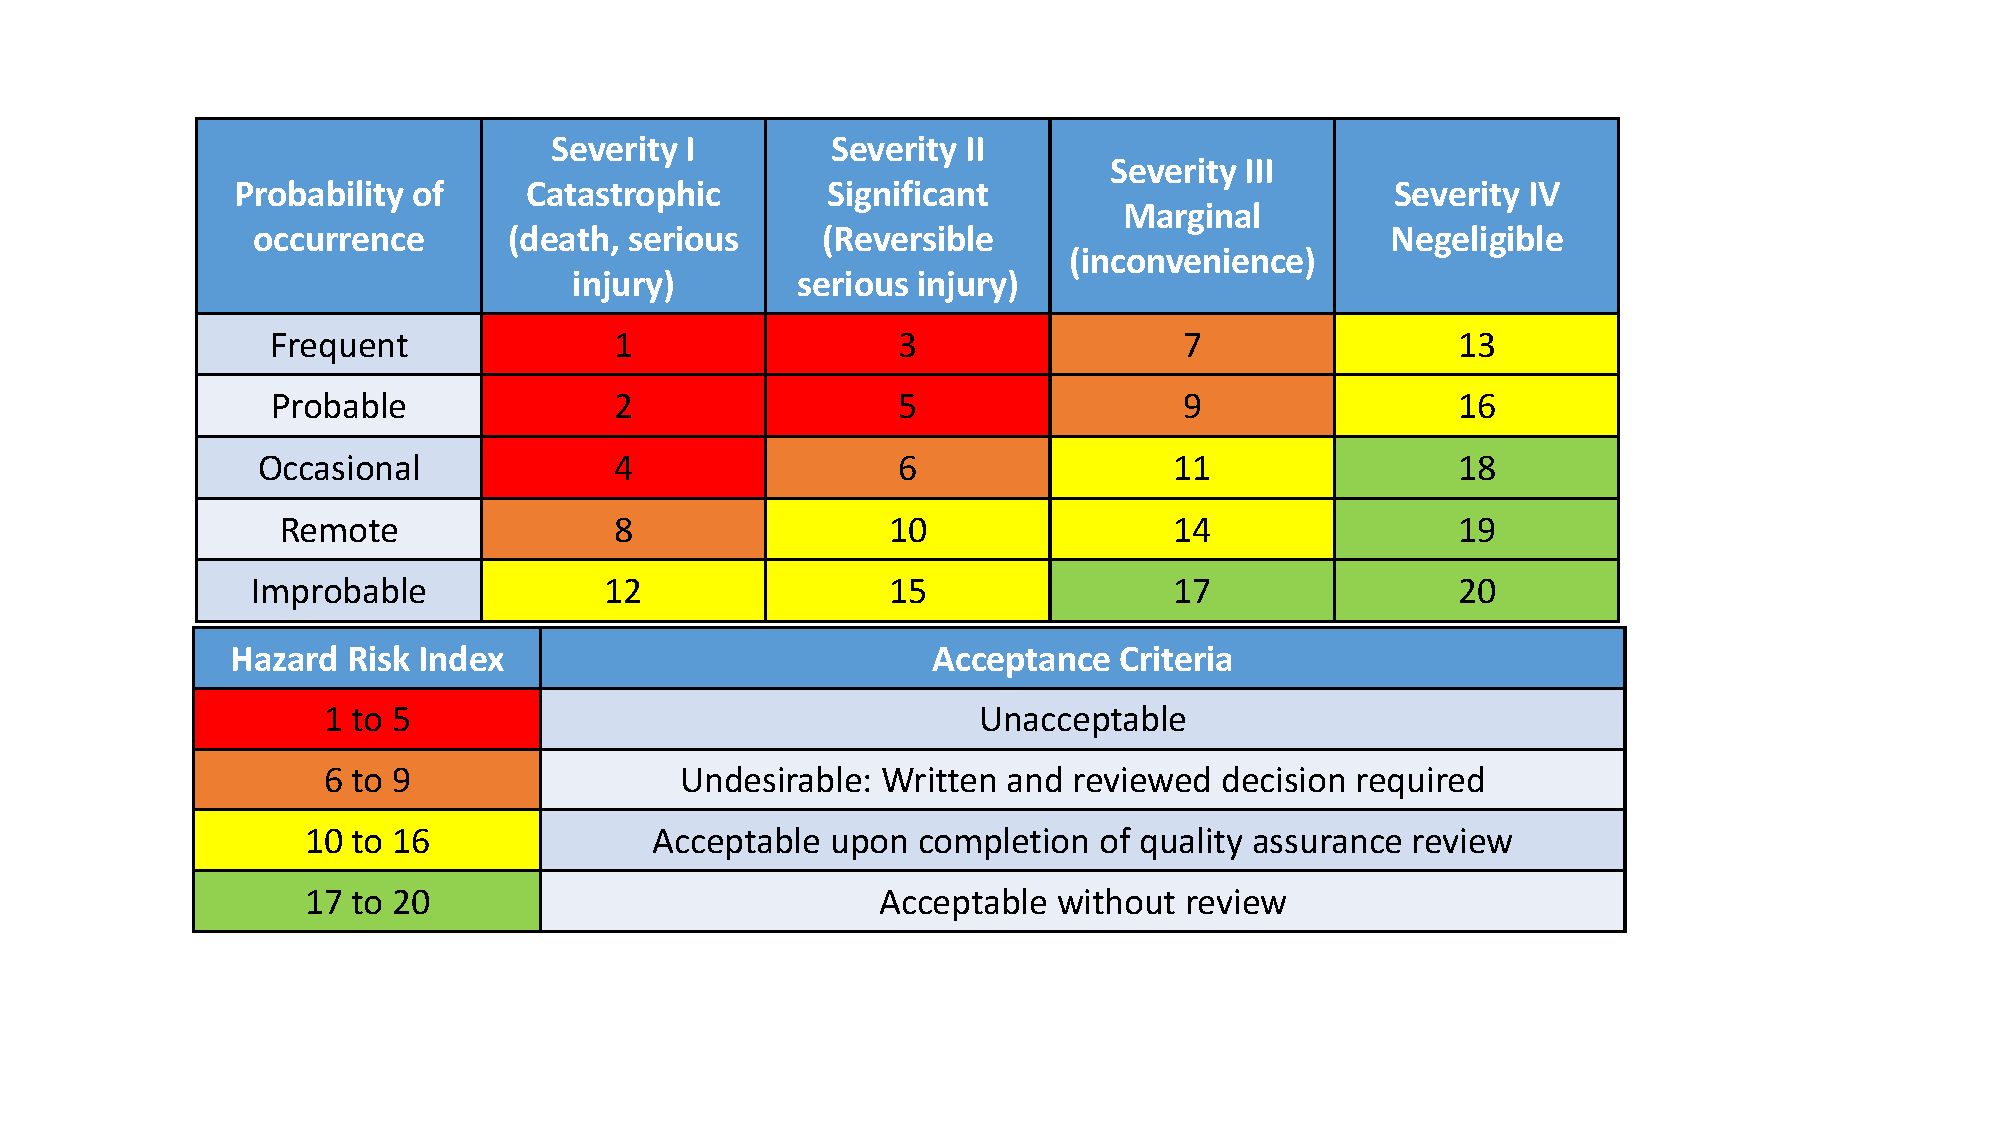
\includegraphics[width=\textwidth]{figs/risk_analysis.pdf}
		\caption{Top table: Risk index according to occurrence and severity. Bottom table: Risk control using risk index}
		\label{fig:risk_ana}
\end{figure}

After the fault tree has been constructed, probabilities for the initial faults are analyzed bottom up to calculate the probability of each hazard. The technique is called Failure Mode and Effects Analysis (FMEA). Then the risks are evaluated by assigning risk index to each hazard according to their occurrence and severity (\figref{risk_ana}). After the risks are evaluated, different activities are required to mitigate the risks according to the risk index. The risks are then be re-evaluated to calculate the residual risk and analyze the risk/benefit. This is part of the risk control process. FMEA is good at exhaustively cataloging initiating faults, and identifying their local effects. It is not good at examining multiple failures or their effects at a system level.

\subsection{Pre-Market Evaluation with Clinical Trials}
Regardless of how rigorous the risk management and the device development process are, the devices have to be able to achieve their design goal on the real patient, which can only be evaluated within its physiological environment. Devices that have high risk factors, including the closed-loop medical devices, are required to submit clinical evidence for their safety and efficacy, often in form of clinical trials. In clinical trials, the devices are used on a preselected population of patients following carefully-designed protocols. The goal of a medical trial, in part, is  to obtain unambiguous results for the primary question of the trial which can support the safety and/or efficacy of the devices. However, conducting clinical trials is very time consuming and expensive, and risks found during clinical trials are very expensive to fix (\cite{trialcost}). 

To address this \textbf{safety gap} between ensuring the device satisfies its therapeutic requirements with the patient-in-the-loop and testing its software specifications, new approaches for closed-loop validation of the device software within the physiological context are needed - this is the primary focus of this article.
%Through the course of the 1980s, software began to play an increasing role in medical devices. Software, as it turns out, is one of those technologies not anticipated by prior regulation, and was waiting for its disaster to prompt regulatory action. It wasn't until the 1980s when a number of cancer patients received massive X-ray overdoses during radiation therapy with the Therac-25 linear accelerator. This lead to a number of investigations, perhaps the most thorough of which was that of \cite{therac}, which was rich with identified ways software could go wrong. Inadequate testing, dangerous code reuse, configuration management issues, inadequate manufacturer response, and failure to get to the root cause of the problem were among the leaders of the problems identified. The Therac-25 was an eye-opener for the FDA and legislators, and resulted in the Safe Medical Device Act of 1990. This finally required closer medical device tracking, post-market surveillance and recommendations on development, testing and validation of medical device software. \todo{Are these useful?}

%\subsection{Pre-market Submission Process}

%There are two processes through which a medical device can enter the market in U.S.: the Premarket Notification, also known as 510(k) \cite{510k}, and the Pre-Market Approval (PMA) \cite{PMA}. In a 510(k) submission the device manufacturers are only required to provide evidence that the device is \emph{substantial equivalent} to a \emph{predicate device}, which has been approved for the market. Therefore, the 510(k) submission does not directly require clinical evidence for the safety and effectiveness of the device, thus it is suitable for mostly low-risk devices like Class I and Class II devices.  The Pre-Market Approval (PMA) submission is a more stringent regulatory process in which direct clinical evidence is required to prove the safety and effectiveness of the device. However, not all Class III devices are subject to PMA submission. If a Class III device clears the 510(k) process and FDA has not requested PMA for that device, the device is still cleared for market release. A study shows that for Class III devices which PMA has been requested, the levels of evidence varies. Only 40\% of the PMA submissions are supported by controlled clinical trials, which provide the most rigorous clinical evidence \cite{cert_prob}. The lack of quality evidence is usually due to the high cost of the controlled clinical trials.

%\subsection{Safety and Efficacy Evidence}

%\todo[inline]{List of software standards}

%The FDA currently does not request or review the medical device software during pre-market submission. This is currently satisfied by the documentation of code inspections, static analysis, module-level testing and integration testing and their purpose is to establish ``reasonable assurance of safety and effectiveness''. These tests however fail to check for the correctness of the software and are largely open-loop tests that do not consider the context of the patient. Software is reviewed by the FDA only in the incident of a device recall. Software-related recalls are often issued in the form of \emph{Safety Alerts} by the %%%%%Food and Drug Administration (FDA) 
%FDA such as ``Safety alert - Pacemaker may revert to VVI mode at 70 beats/min if programmed to one of several specific ventricular pulse widths" (\cite{medstats}).


%\section{Challenges to Develop Safe Medical Device Software}
%\subsection{Safe Development Process vs. Safe Product}
%Conformance to the safety standards provides strong confidence on a safe development process. The belief is that a well-planned, systematic engineering process produces more reliable devices, especially if software is a component of the device (\cite{med-book}). However, there is no guarantee that safe process always yield safe devices. Recently there is growing interest on enforcing safety and efficacy evidence for the device itself. \cite{Wassyng} Due to the large variety of medical devices, there does not exist general safety and efficacy requirements that can be written into standard. As the result, evidence for product safety and efficacy varies in quality and organization. Assurance cases \cite{} have been proposed to help constructing safety arguments and organizing safety evidences. Assurance cases are currently "Recommanded" by FDA during regulation submission. (\cite{})


%\subsection{Multiple Stakeholders}
%For each medical device, there are 4 stakeholders: the regulator, the device manufacturer, the medical professional and the patient. All parties have the incentive to ensure the safety and efficacy of the device. With current regulation framework, the evidence for safety 
%\begin{figure}[t]
		%\centering
		%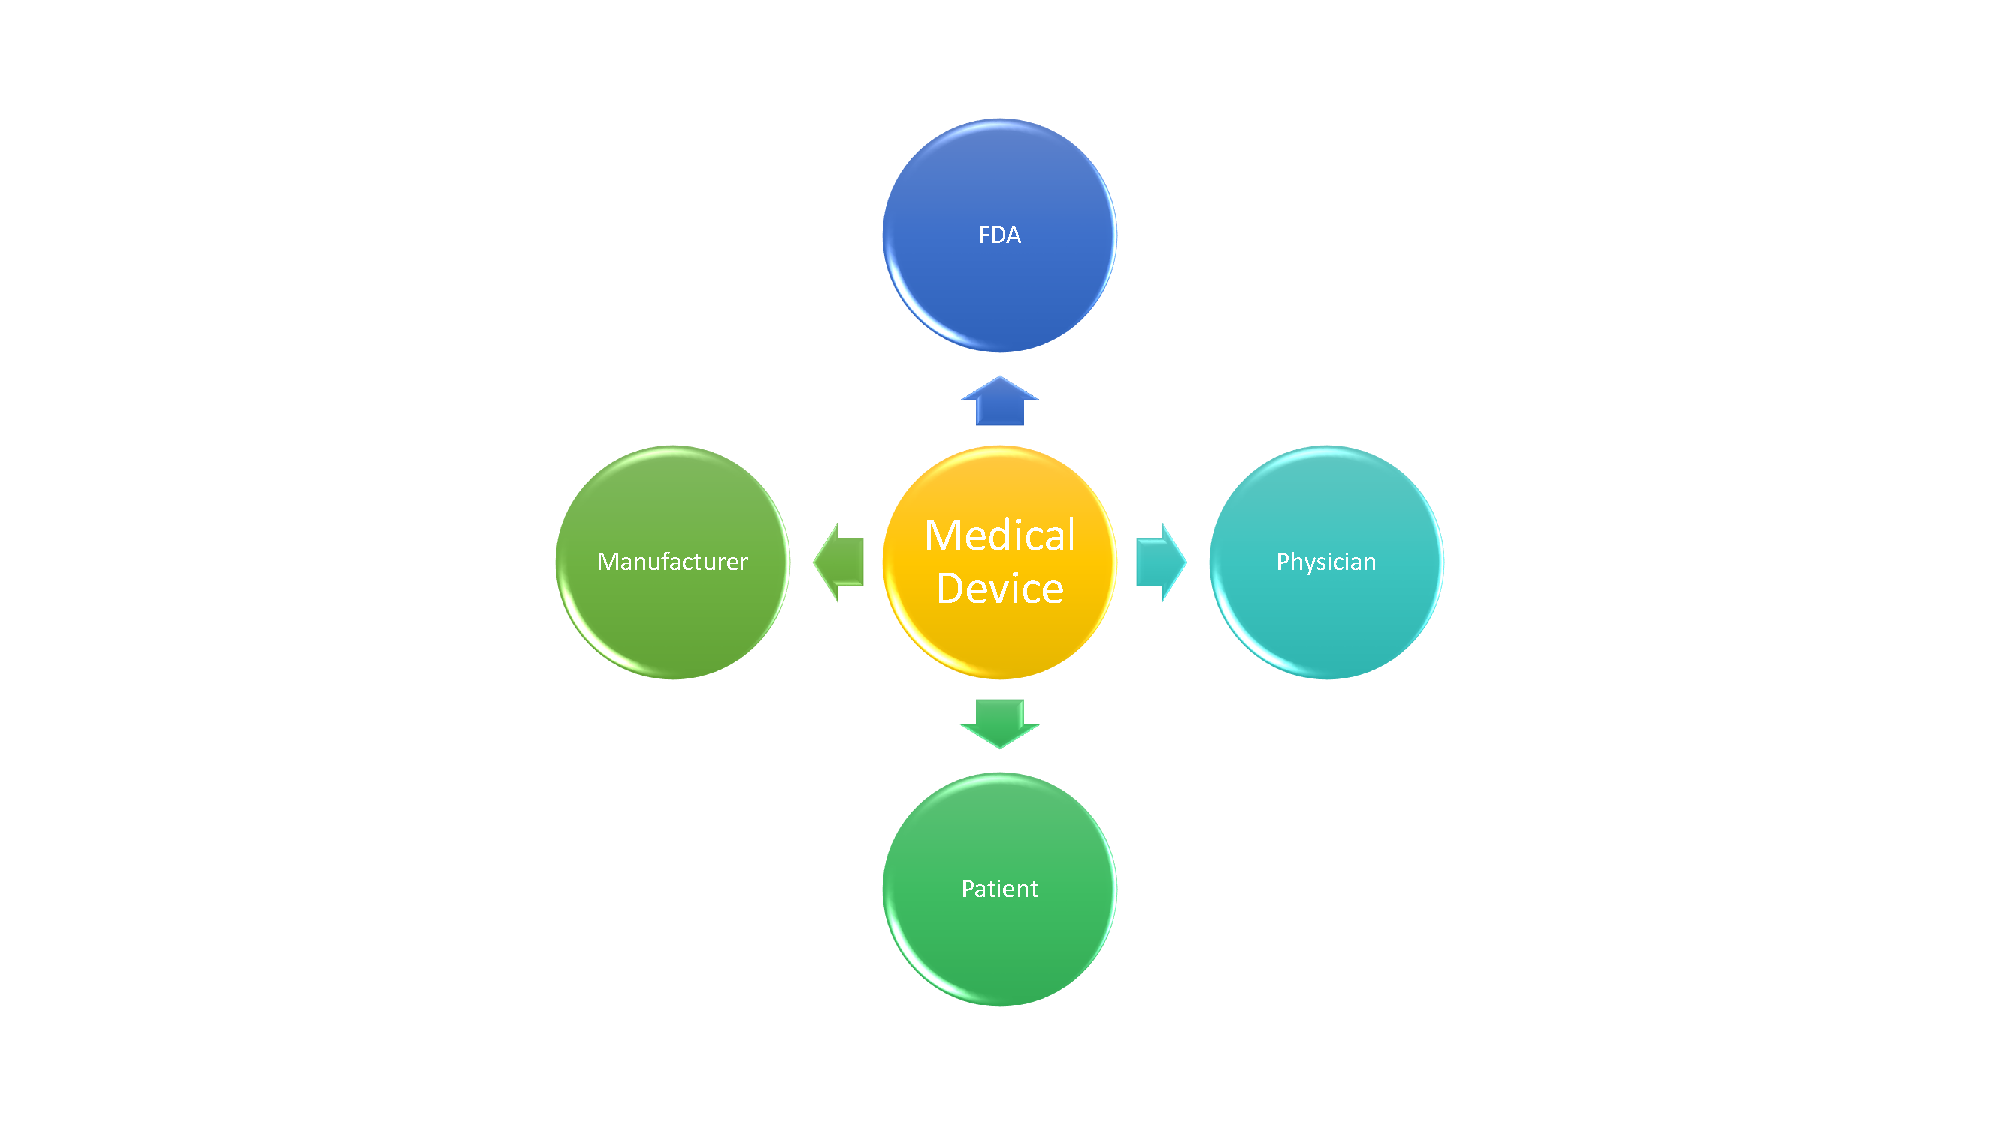
\includegraphics[width=0.8\textwidth]{figs/stakeholders.pdf}
		%\caption{\small Figure of current medical devices}
		%\label{fig:Cur}
%\end{figure}
%However, the medical domain presents its own unique set of challenges:\\
%\textbf{1. Closed-loop context:} Current evaluation of devices is open-loop and is unable to ensure the device never drives the patient into an unsafe state. Medical device testing and validation must thus be within the closed-loop context of the patient physiology. The context of the patient is a function of both the environment and the input from the device controller and must be captured by the device evaluation process.\\ 
%\textbf{2. Patient models:} There is a scarcity of patient models and clinically-relevant simulators for device design (\cite{pat-model}). High-fidelity models of interaction between the patient and device are needed to evaluate the safety and efficacy of device operation. Furthermore, these models must integrate the functional and formal aspects so that testing and verification are evaluated for the same patient states.\\
%\textbf{3. Adaptive patient-specific algorithms:} The therapy offered by the device must adapt to the environment and specific patient's condition. There is a need for validation algorithms to ensure that device control and optimization can cover large classes of patient conditions. 

%\section{The FDA and Medical Device Software}
%Before we delve into the current state of medical device software, it is useful to understand the evolution of the regulatory environment. 




%\section{Current Testing, Validation and Verification Approaches}
%In order to facilitate the early detection and correction of any software defects, the FDA has focused on infusion pumps due to the large number of recalls. In April 2010, the FDA began the ``Infusion Pump Improvement Initiative" which offers manufacturers ``the option of submitting the software code used in their infusion pumps for analysis by agency experts prior to premarket review of new or modified devices." 	\cite{}
%
%An effective software verification methodology is therefore needed for the risk analysis and certification of medical device software during the pre-market submission phase. While formal methods of verification are used for medical device software (\cite{challenge, challenge2, challenge3}), testing continues to be required because it can expose different kinds of problems (e.g. compiler bugs), can examine the program in its system context, and increases the diversity of evidence available. Testing for medical device software currently is ad hoc, error prone, and very expensive. Traditional methods of testing do not suffice as the test generation cannot be done independently of the current state of the patient and organ. The primary approach for system-level testing of medical devices is unit testing using a playback of pre-recorded electrogram and electrocardiogram signals (\cite{testing_imd, Vip}). This tests if the input signal triggers a particular response by the pacemaker, but has no means to evaluate if the response was appropriate for the patient condition. Furthermore, this approach of ``tape testing''\Hao{elaborate} is unable to check for safety violations due to inappropriate stimulus by the pacemaker. Pacemaker Mediated Tachycardia (PMT), a condition that is described later in this paper, is a strong example of why we need a model of the heart such as the one presented in this paper, which can be used for closed-loop system analysis. 
%PMT is a condition where the pacemaker inappropriately drives the heart-rate toward the upper rate limit. With a tape test, PMT would not occur and the response of the pacemaker could be classified as appropriate therapy.
%\begin{figure}[t]
		%\centering
		%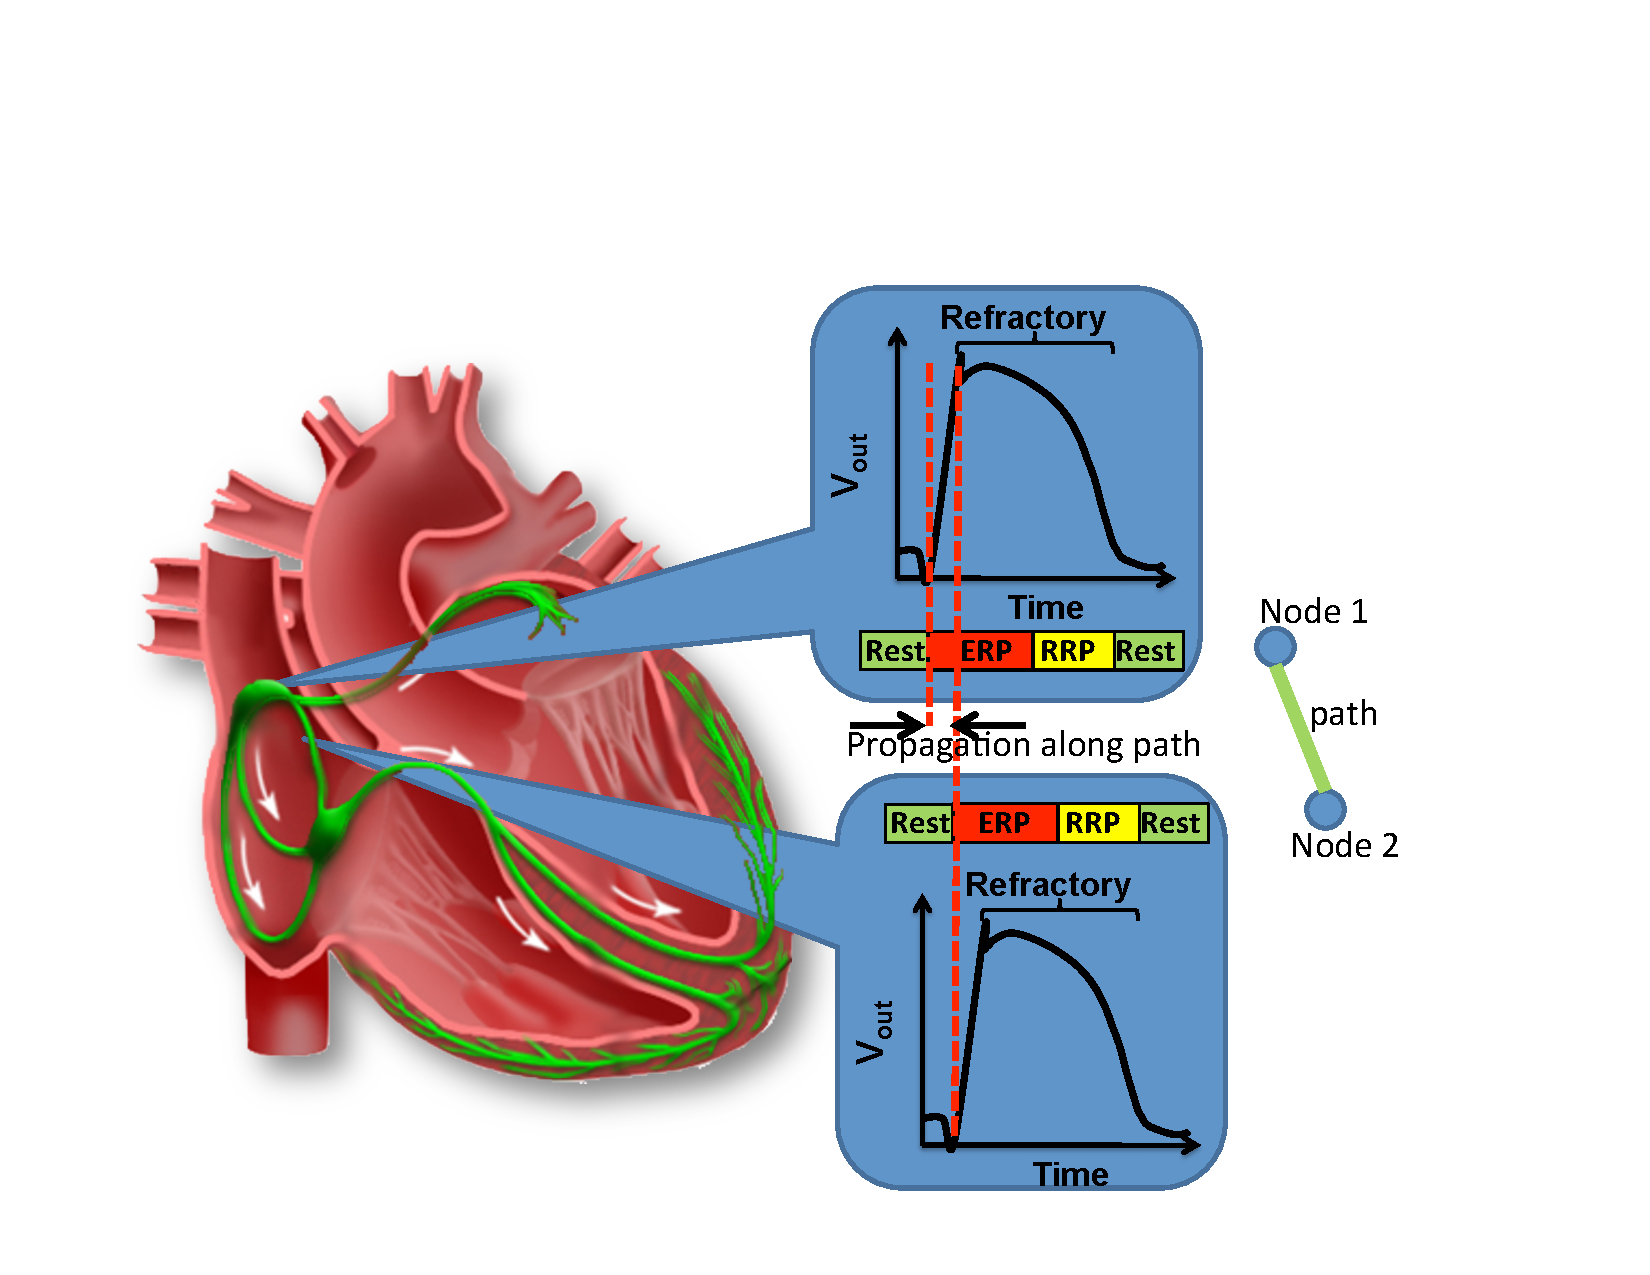
\includegraphics[width=0.8\textwidth]{figs/heartmodel.pdf}
		%%\vspace{-5pt}
		%\caption{\small By extracting timing and electric conduction information we model the signal activation, refractoriness and propagation across the heart tissue as a set of node and path automata.}
		  %%\vspace{-15pt}
		%\label{fig:heartmodel}
%\end{figure}
%As the testing environment (i.e., patient condition) is not entirely under the control of the tester, the problem changes significantly as a degree of nondeterminism is introduced in the process. Implantable medical devices are a primary example of Medical Cyber-Physical Systems where the safety and efficacy of the device and device software must be evaluated within a closed-loop context of the patient. The key challenge is in the generation of physiologically relevant tests such that the device does not provide inappropriate therapy, and does not adversely affect the safety of the patient. In addition, test generation must be interactive and adaptive such that the previous test stimulus affects the current state of the patient. The test generator must consider the current state when generating the next input in a way that advances the purpose of the test. The problem becomes one of the controller synthesis problems and cannot be addressed by an off-the-shelf model checker~\cite{rushby}.  
   %
%Formal methods have traditionally been used for verification of time-critical and safety-critical embedded systems \cite{form-meth}. Until recently, these methods have not been used for medical device certification. \cite{med-form3} presented the use of Extended Finite State Machines for model checking of a resuscitation device. Formal techniques have also been applied to improve medical device protocols (\cite{med-form2}) and safety (\cite{med-form1}), but the authors either used a simplified patient model or did not model the patient at all. 
\section{Model-based design to improve medical device safety}
With the deluge of software-based closed-loop medical devices in the coming years, relying on clinical trials as the only closed-loop evaluation method to identify risks rooted in device software is not scalable. Model-based design and virtual integration have been proposed and applied in other industries like automotive and avionics (\cite{autosar, avsi}), and can potentially help during the development process and provide extra confidence to the device before conducting clinical trials. However, unlike man-made systems like automobiles and aircrafts, physiological systems are less understood with larger variations for the type and degree of patient conditions. The lack of faithful models of physiological environment of the closed-loop medical devices is one of the reason that model-based design is not well-adopted in the medical device industry. 
\begin{figure}[t]
		\centering
		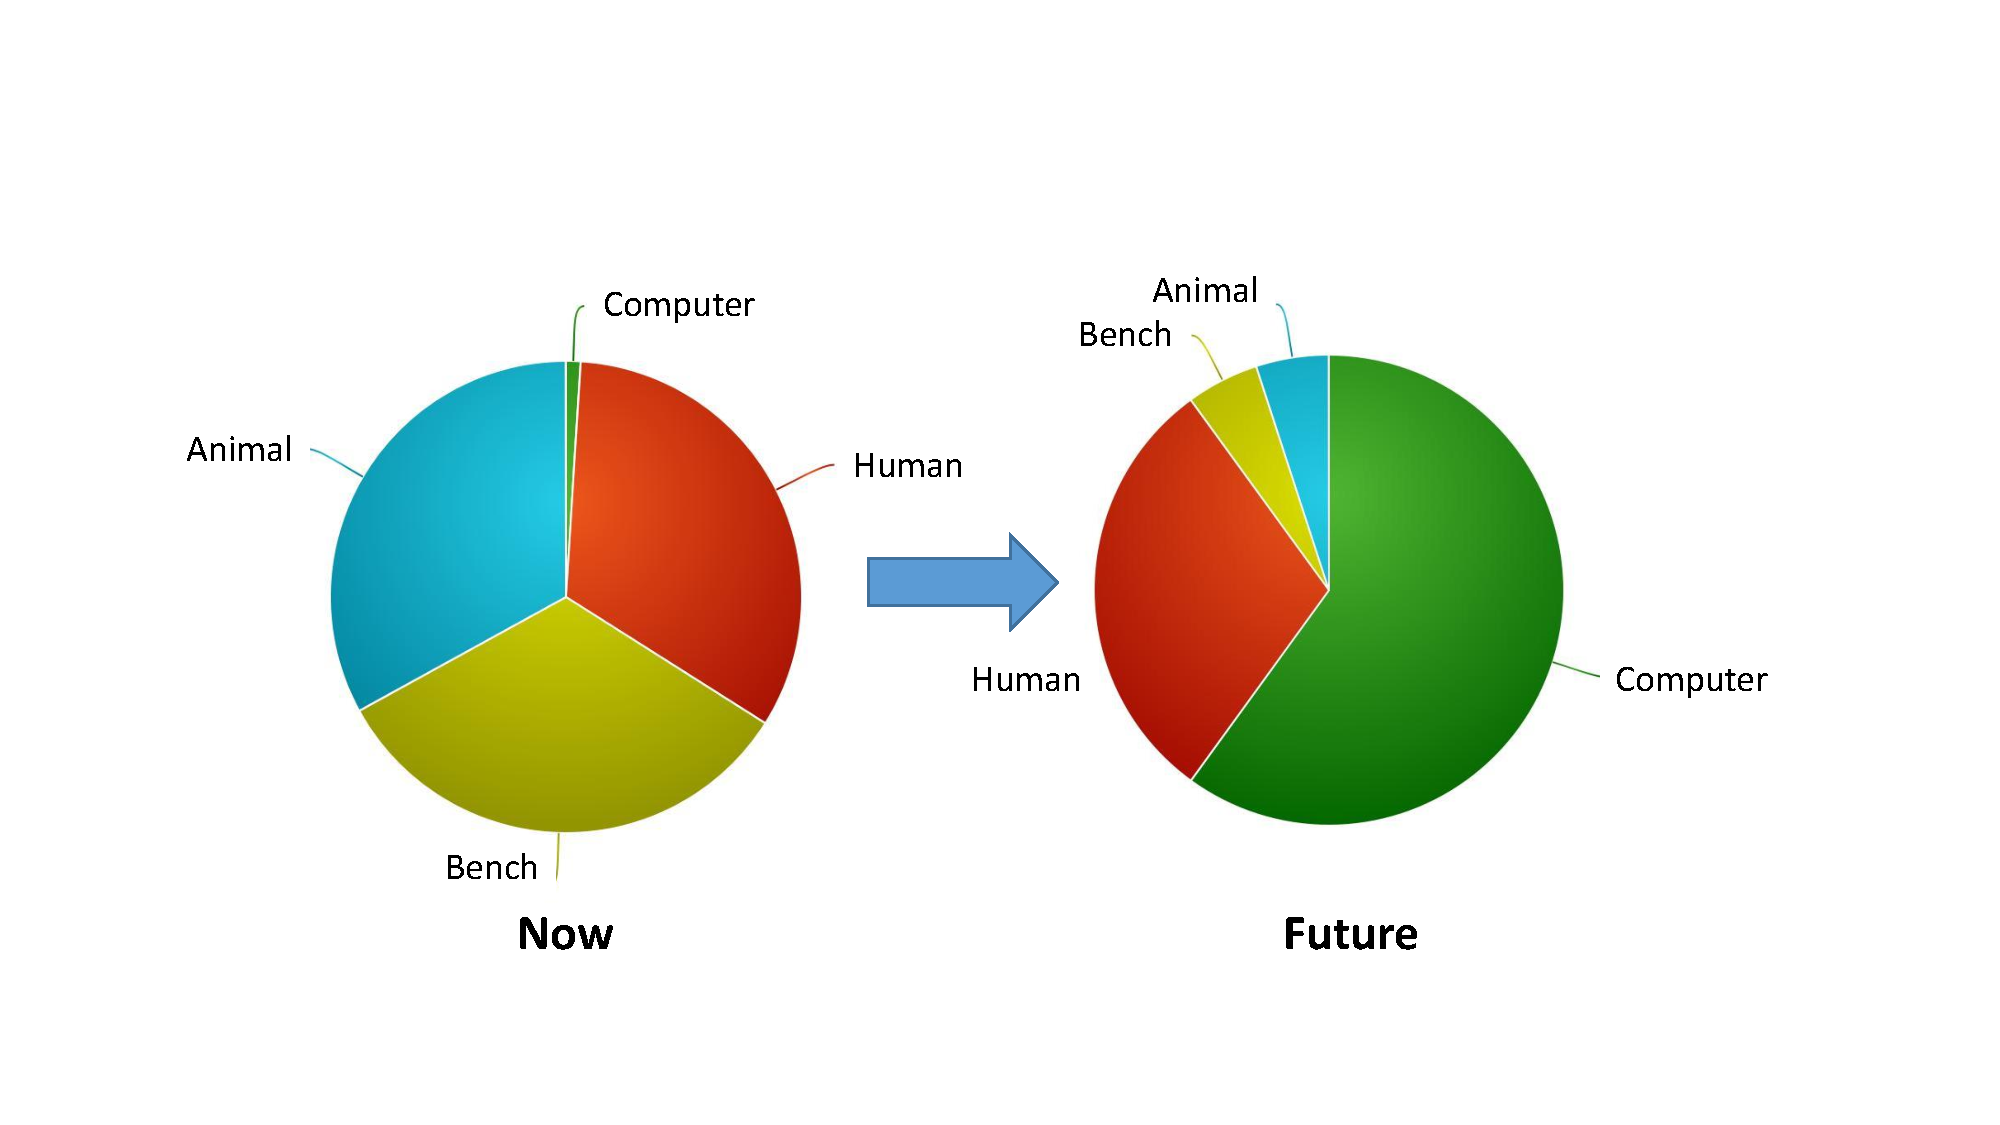
\includegraphics[width=\textwidth]{figs/MDIC.pdf}
		\caption{\small Percentage of computer simulation is expected to increase as safety and effectiveness evidence of medical devices}
		\label{fig:MDIC}
\end{figure}

As computational models of human physiology are developed, they can be used to interact with closed-loop medical devices or their models. The FDA is starting to recognize in-silico modeling and simulation as regulatory-grade evidence for device safety and efficacy. For example, \cite{pancreas_paul} developed glucose-insulin models that can be used to evaluate control algorithms for artificial pancreas devices which can sense blood glucose and deliver insulin. Simulation results with the models have been recognized by FDA to replace animal trials, in part, which significantly reduced cost (\cite{pancreas}). With the increasing interest and recognition from the regulators, computer models and simulations are expected to play bigger role as as ``regulatory-grade evidence" evidence in the development of future closed-loop medical devices (\figref{MDIC}).

\section{Contributions}
In this article, we use an implantable cardiac pacemaker as a working example to demonstrate how model-based design can help improve the safety and efficacy medical device software. We demonstrate the application of model-based design in several design activities during the development process, from the perspective of the manufacturer's design validation team. We assume availability of design artifacts including pacemaker design and physiological requirements. By demonstrating the process of developing verified models to generate verified code, the results of our model-based closed-loop evaluation should be able to support the device's safety and efficacy requirements during the regulation process.
\begin{figure}[t]
		\centering
		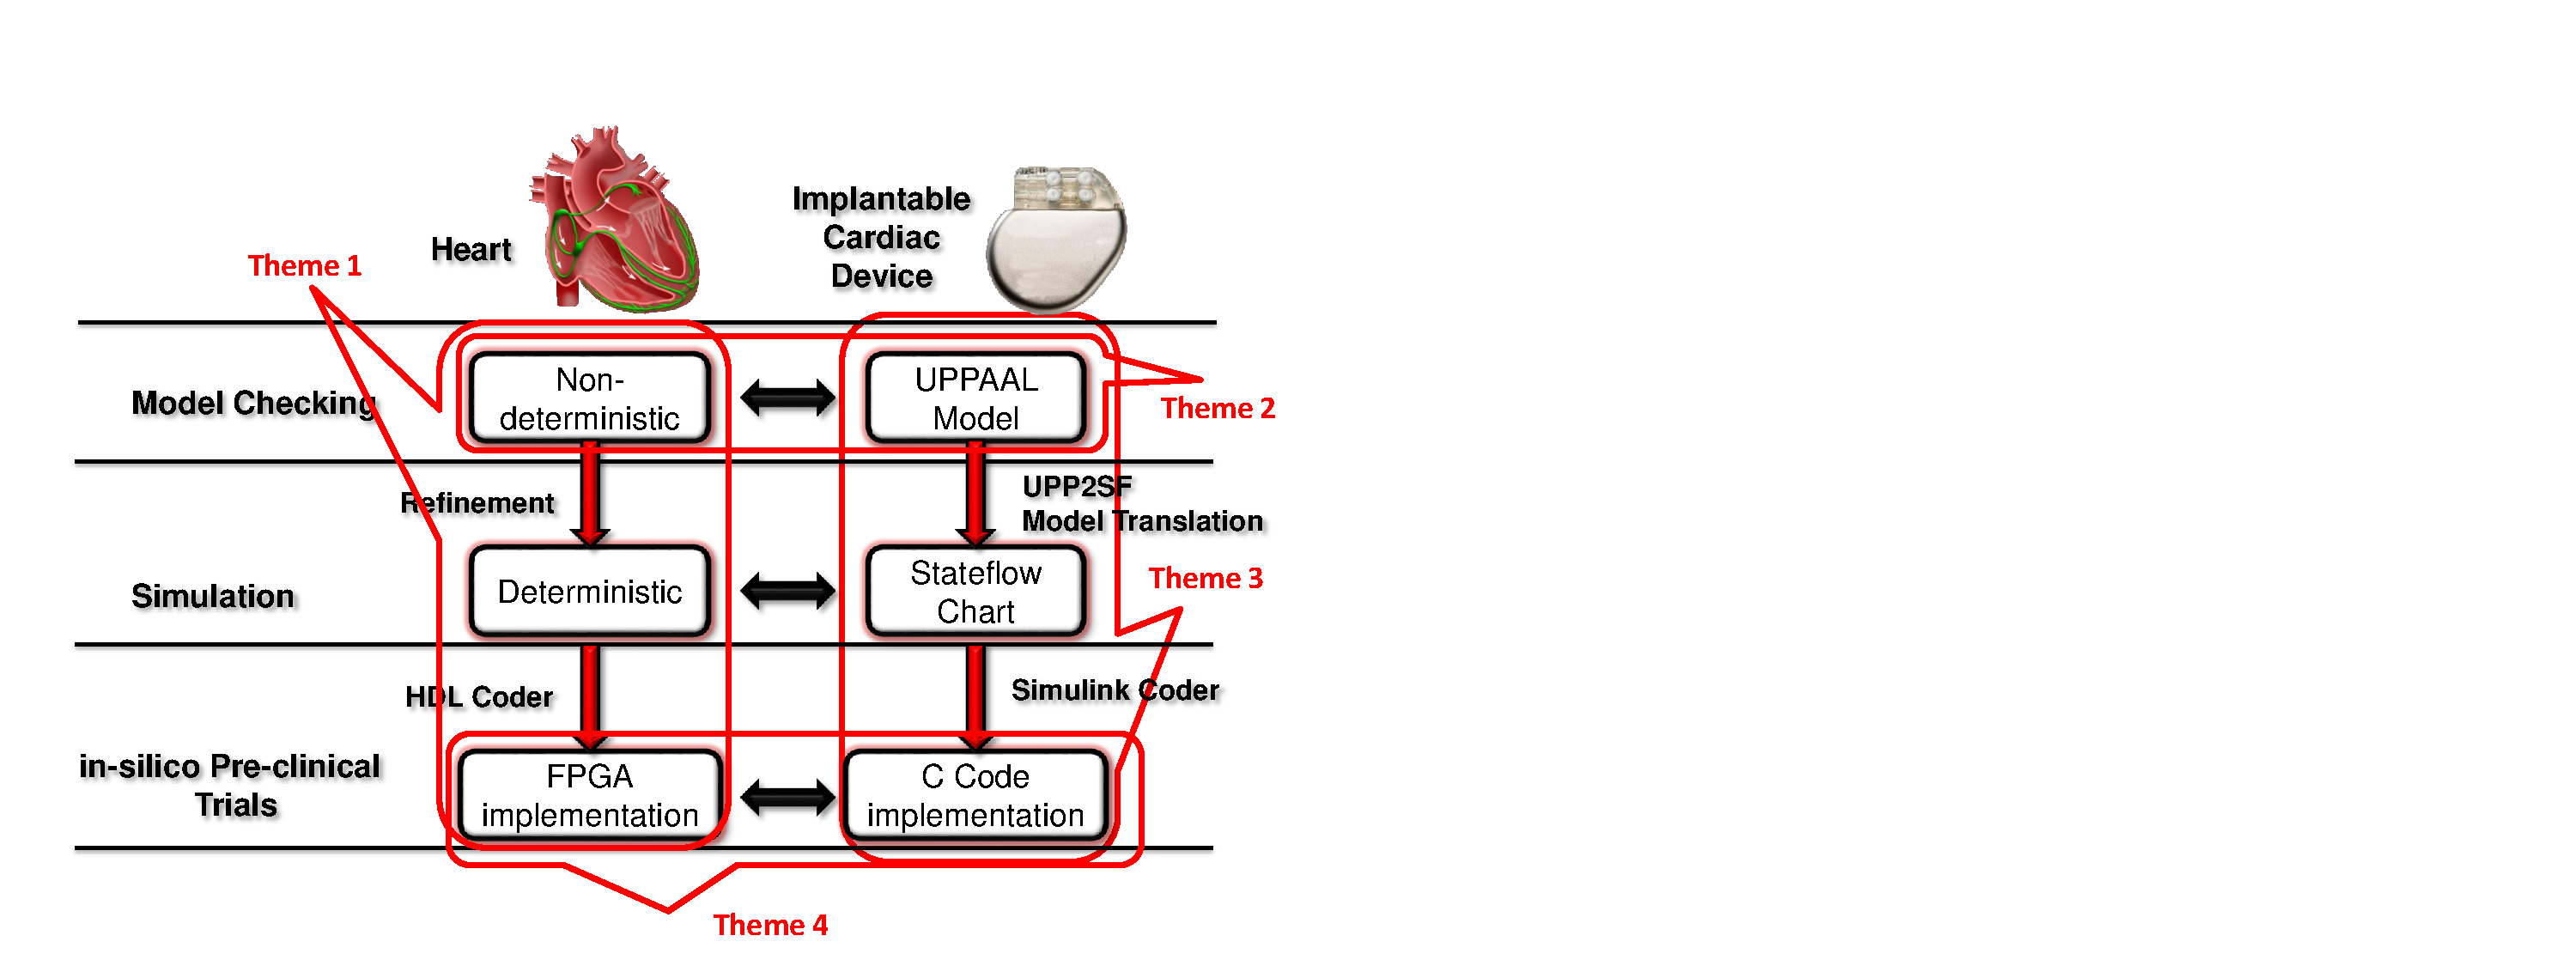
\includegraphics[width=0.9\textwidth]{figs/model_based_b.pdf}
		%\vspace{-5pt}
		\caption{\small Model-driven design for verified models to verified code for the closed-loop heart and pacemaker system}
		  %\vspace{-15pt}
		\label{fig:modeling_overview}
\end{figure}

Our proposed model-driven design for closed-loop medical devices (\figref{modeling_overview}) begins with developing heart models that can interact with real and modeled pacemakers (\cite{VHM_proc}). In Chapter 2, we introduce our heart models for closed-loop  \emph{model checking} and  \emph{testing} of implantable cardiac devices, and the rationale for the difference between heart models used in these two applications. For closed-loop evaluation, the heart models have to be able to represent and respond under different physiological conditions. The heart models are available in different formalisms to interact with the pacemaker design in closed-loop across different design stages. In Chapter 3, we validate the heart models and discuss how to identify model parameters from patient data so that the heart model can represent different physiological conditions. 

In Chapter 4, we introduce the pacemaker software specification which is referenced from a dual chamber pacemaker design from Boston Scientific (\cite{compass}). The software specification is converted to an abstract formalism called \emph{Timed Automata} (\cite{timed_automata}). The timed automata model of the pacemaker will be the starting point for our model-based analysis and implementation. In Chapter 5, we identify two basic hazards for pacemaker and use the UPPAAL model checker (\cite{uppaal}) to evaluate whether the hazards have been reasonably mitigated. With the help of heart models introduced in Chapter 2, we are able to cover the closed-loop behaviors of large variety of heart conditions so that we can evaluate whether there exists any known and even unknown mechanism to induce hazards (\cite{STTT13}). Pacemaker and heart models used in model-checking are abstract as model checkers do not scale well with increased model complexity. So complex dynamics of the heart and pacemaker are not captured at this stage. 
\looseness1

In Chapter 6, we describe the development of an automatic model translation procedure to translate models from UPPAAL to Stateflow (\cite{stateflow}) to ensures that abstract models used for verification over-approximate the more detailed models used downstream (\cite{RTAS12}). The Stateflow model of the pacemaker is then evaluated with heart models with relatively complex dynamics (\cite{vhm_ecrts10, vhm_embc11,vhm_iccps11}). Once the detailed models pass simulation-based testing with closed-loop dynamics, they are automatically generated into code and are subject to platform-level integration testing (\cite{vhm_website}). This model-driven design approach ensures the closed-loop safety properties are retained through the design toolchain and facilitates the development of verified software from verified models.

%The contribution of this effort is three-fold: (a) We developed an integrated functional (i.e., clinically-relevant) and formal (i.e., timed automata based) Virtual Heart Model  (VHM) (see \figref{heartmodel}) and a pacemaker device model for interactive and clinically relevant test generation.  (b) We provide a set of general and patient condition-specific pacemaker software requirements to ensure the safety of the patient is met under all cases, and (c) We provide a means to test and verify the closed-loop system over a variety of basic operation tests where the heart rate must be maintained, the atrial-ventricle synchrony must be enforced and complex closed-loop tests, where the pacemaker must not initiate tachycardia or perform improperly during lead displacement. With this approach of model-based testing, an executable functional model of the pacemaker is created at an early stage in the development process. This model-based methodology is an early step in addressing the urgent need for pre-market evaluation of medical device design and certification.

\vspace{-10pt}
\section{Useful terminologies for often misinterpreted terms}
Ensuring the safety of complex medical devices has drawn interest not only from stakeholders like regulators and industries, but also medical professionals and academia. Different communities have different interpretations over certain terminologies, often causing misunderstandings. In this paper we adopt the terminologies from the regulation perspective, so that the results we have fit into the regulation framework. Most of the definitions are referred from the FDA guideline document General Principles of Software Validation (\cite{fda2}). Below are several terminologies that we use throughout the paper which worth clarifying.
\vspace{-5pt}
\subsection{Requirements vs. Specifications}
By the definition of FDA (\cite{fda3}), the requirements of a system describe \textbf{what} the system should achieve and the specifications of a system describe \textbf{how} the system is designed to satisfy the requirements. For example, a requirement for an autonomous car is "The car should not hit objects". The corresponding specification can be "brake if the speed of the car is greater than $x$ and the distance to the object is less than $y$". We can see that a car satisfying its specification may not satisfy the requirement (e.g. when the car is driving too fast or the obstacle pops up right in front of the car). In this paper, we use the word requirement in particular to denote the intended uses of the medical devices to improve physiological conditions.

\subsection{Validation vs. Verification vs. Testing}
As defined in \cite{fda2}, software validation is the confirmation by examination and provision of objective evidence that:
\begin{enumerate}
	\item software specifications conform to user needs and intended uses, and 
	\item the particular requirements implemented through software can be consistently fulfilled
\end{enumerate}
The first aspect ensures the device is safe and effective. The second aspect maintains the traceability of requirements throughout the development life cycle.
Software verification fulfills the second aspect of software validation by "providing objective evidence that the design outputs of a particular phase of the software development life cycle meet all of the specified requirements for that phase. "
\begin{figure}[t]
		\centering
		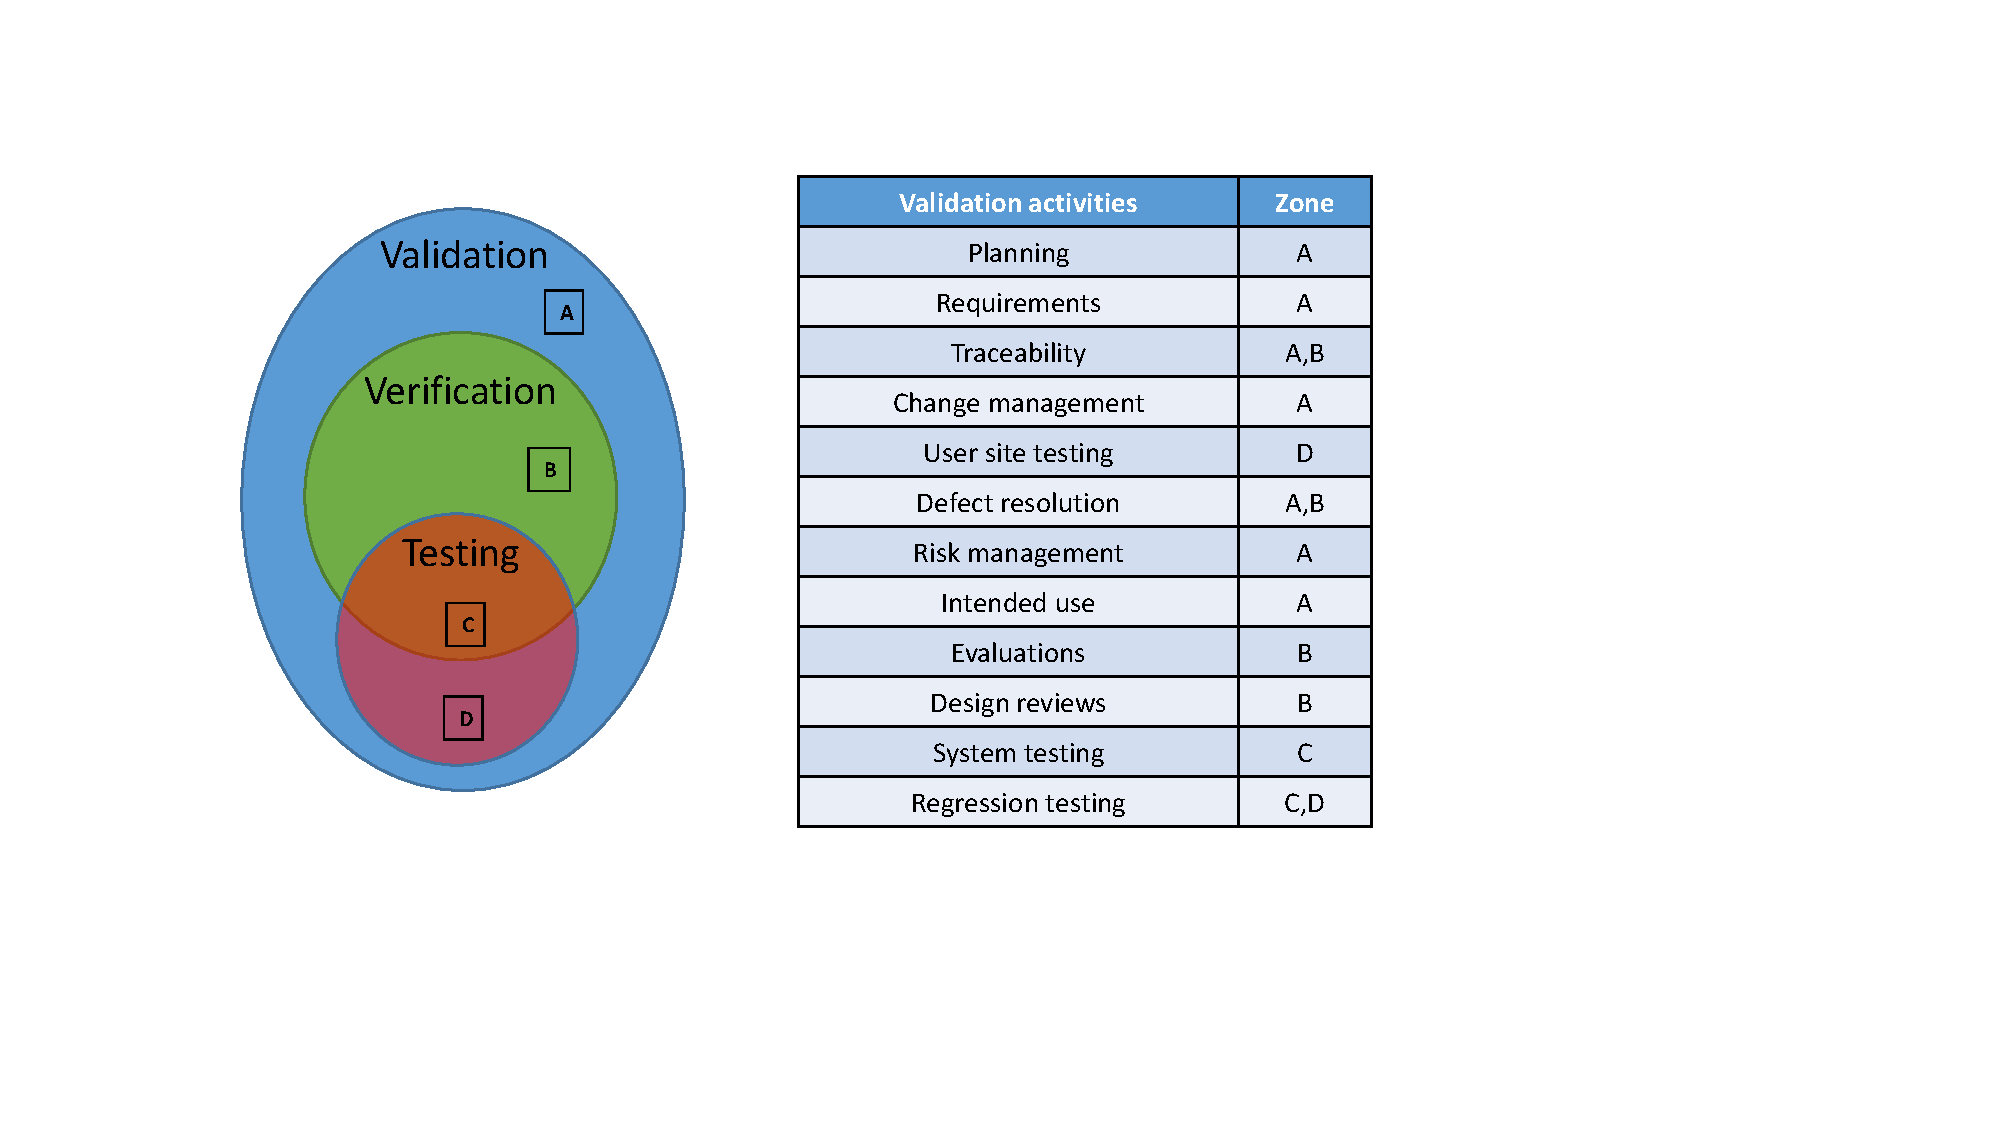
\includegraphics[width=\textwidth]{figs/validation.pdf}
		\caption{Validation activities during the software development life cycle (\cite{Vogel})}
		\label{fig:validation}
\end{figure}

Testing is the technique that can be used for validation and/or verification. \figref{validation} illustrates the relationship between validation, verification and testing, and different activities during the software development life cycle to ensure the safety and effectiveness of the software.
\subsection{Closed-loop vs. Open-loop Evaluation}
In open-loop evaluation, i.e. open-loop testing, input sequences are send to the system and system outputs are compared with expected outputs. In open-loop testing, the system outputs do not affect the inputs afterward. In closed-loop evaluation, the environment of the system is taken into account. System outputs affect the state of the environment and thus affect the input sequences. For closed-loop medical devices, clinical trials are currently the most common closed-loop evaluation method. Enable closed-loop evaluation at model level requires models of the environment, which is human physiology for closed-loop medical devices.

Closed-loop evaluation accomplishes two goals in model-based design: 1) It enforces environmental constraints so that the test space is smaller and the test cases have physiological relevance. 2) Execution traces can be better interpreted as the physiological models encode domain knowledge. 
%%Through each of the chapters to follow, we cover different aspects of modeling the physiological system and the device, validating the models, running model checking on the closed-loop system and testing the deterministic systems derived from the abstract models. With the goal of 

%%The US Food and Drug Administration defines medical device an instrument, apparatus, implement, machine, contrivance, implant, in vitro reagent, or other similar or related article, including a component part, or accessory which is:
%%\begin{itemize}
%%	\item recognized in the official National Formulary, or the United States Pharmacopoeia, or any supplement to them
%%	\item intended for use in the diagnosis of disease or other conditions, or in the cure, mitigation, treatment, or prevention of disease, in man or other animals, or
%%	\item intended to affect the structure or any function of the body of man or other animals, and which does not achieve any of its primary intended purposes through chemical action within or on the body of man or other animals and which is not dependent upon being metabolized for the achievement of any of its primary intended purposes."
%%\end{itemize}
\chapter{A Motivating Example: Dual Chamber Pacemaker}
In this chapter we introduce a dual chamber pacemaker specification.
It is used throughout the thesis to demonstrate how different model-based techniques can be used to validate the safety and efficacy of the pacemaker.
\section{Physiology Basis of the Heart and the Pacemaker}
First, we use this small section to introduce the physiology basis of the heart and the application of implantable cardiac devices. Readers with knowledge of this subject can skip to the following sections.
\subsection{Blood Circulation System}
The heart is the "motor" for blood circulation within our body. The heart has two ventricles which pump the blood out of the heart, and two atria which gather blood from the body and pump them into the ventricles. (\figref{circulation}.(a)) There are two circulations through the heart: the \emph{Pulmonary circulation} and the \emph{Stemic circulation}. In the pulmonary circulation, the right atrium collects oxygen-depleted blood from all over the body and pumps it into the right ventricle. The right ventricle then pumps low-oxygen blood to the lungs. The blood gets oxygenated in the lungs and gathers into the left ventricle. In the stemic circulation, the oxygenated blood in the left atrium is pumped into the left ventricle. The left ventricle pumps the blood to the rest of the body and the heart itself. After the body extracts the oxygen from the blood and injects carbon dioxide, the oxygen-depleted blood then flows back to the right atrium.
\begin{figure}[!t]
\centering
		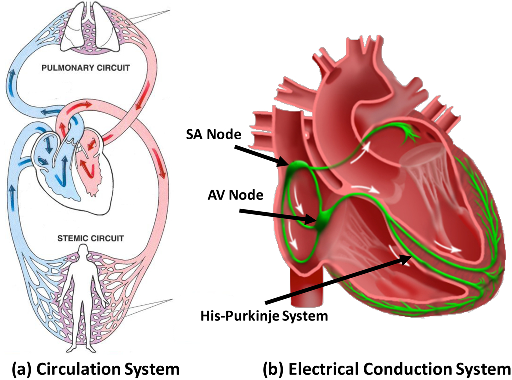
\includegraphics[width=0.9\textwidth]{figs/circulation.pdf}
		
%\vspace{-10pt}
\caption{\small (a) The circulation system. (b) Electrical Conduction system of the heart}
\label{fig:circulation}
%\vspace{-15pt}
\end{figure} 
\subsection{Electrical Conduction System of the Heart}
The oxygen demand of the body changes during different activities. For example, the demand is higher while running and lower while sleeping. To satisfy these demands, the heart muscles in the atria and the ventricles have to contract with certain frequency and in accordance to optimize the \emph{Cardiac Output}, which refers to the volume of blood pumped by the heart per minute (mL blood/min). The coordinated contractions of the heart muscles are governed by the electrical conduction system of the heart (\figref{circulation}.(b)) A \emph{Normal Sinus Rhythm (NSR)} is the healthy heart rhythm which provides efficient blood flow. During a NSR, electrical signals are periodically generated by the \emph{Sinoatrial (SA) node} in the upper right atrium, which acts as the intrinsic pacemaker of the heart. The signals conduct throughout both atria and trigger muscle contractions to push blood into the ventricles. After a long conduction delay at the \emph{AV node} so that both ventricles are fully filled, the signals conduct through fast-conducting \emph{His-Purkinje} system to trigger almost simultaneous contractions of the ventricles and pump blood out of the ventricles. 

Derangement from NSR can result in insufficient cardiac output and thus insufficient oxygen supply to the body and/or the heart itself, which are referred to as \emph{Arrythmia}. Arrhythmia impair the heart's ability to efficiently pump blood and compromise the patient's health. 
Arrhythmia are categorized into so-called \emph{Tachycardia} and \emph{Bradycardia}. Tachycardia features undesirable fast heart rate which can cause inefficient blood pumping. Bradycardia features slow heart rate which results in insufficient blood supply. Bradycardia are due to failure of impulse generation with anomalies in the SA node, or failure of impulse propagation where the conduction from atria to the ventricles is delayed or blocked. 
\subsection{Electrophysiology and Implantable Cardiac Devices}
\label{EP}
The electrical activities of the heart closely couple with the mechanical contractions thus the electrical activities of the heart can be monitored and used to diagnose arrhythmia. The most well-known method is Electrocardiogram (ECG), which measures the integration of electrical activities of the heart measured along different axis on the body surface. The electrical activities can also be directly measured by inserting electrodes through the vein into the heart. The electrodes are placed against the inside heart wall and localized electrical activities can be measured. Physicians can also deliver pacing sequence through the electrodes to explore the heart conditions. This procedure is referred to as Electrophysiological (EP) Testing  (\cite{josephson}) and the signals are referred to as electrograms (EGMs) (\figref{probes}.b). The timing and morphology of the  ECG and EGM signals together are used to diagnose arrhythmia.
\begin{figure}[!t]
\centering
		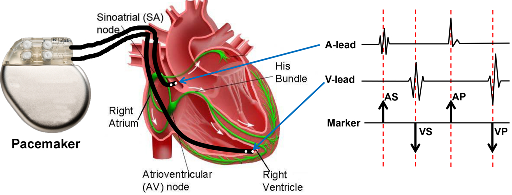
\includegraphics[width=0.9\textwidth]{figs/egm.pdf}
		
%\vspace{-10pt}
\caption{\small (a) Lead placement for a dual chamber pacemaker. (b) Electrogram (EGM) signals measured from pacemaker leads and corresponding internal pacemaker events}
\label{fig:probes}
%\vspace{-15pt}
\end{figure} 

%Implantable pacemakers follow the principle of EP testing. For a dual chamber pacemaker, two leads are inserted into the right atrium and right ventricle, respectively. The pacemaker senses the intrinsic generation and conduction of the electrical signals in the two chambers and deliver electrical pacing when the heart rate and/or atria-to-ventricles conduction interval are abnormal.
The implantable cardiac pacemakers are rhythm management devices designed to treat bradycardia. A typical dual chamber pacemaker has two leads inserted into the heart through the veins which can measure the local electrical activity of the right atrium and right ventricle respectively (\figref{probes}.a). According to the timing between sensed impulses, the pacemaker may deliver electrical pacing to the corresponding chamber to maintain proper heart rhythm.

\section{A Dual Chamber Pacemaker Specification}
In our study, we focus on the implantable pacemaker, which is one of the simpler implantable cardiac devices.
The functionality of a pacemaker is based on the timing of local electrical events, which can be intuitively modeled with timed automata. 
The specifications are based on the algorithm descriptions from Boston Scientific manuals (\cite{compass}) and the functional description released as part of the Pacemaker Challenge (\cite{challenge}). 


The pacemaker is designed for patients with bradycardia (i.e. slow heart rate). Two leads, one in the right atrium and one in the right ventricle, are inserted into the heart and fixed onto the inner wall of the heart. These two leads monitors the local activation of the atria and the ventricles, and generate corresponding sensed events \textsf{(AS, VS)} to its software. The software determines the heart condition by measuring time difference between events and delivers pacing events \textsf{(AP, VP)} to the analog circuit when necessary. The analog circuit then delivers pacing signals to the heart to maintain heart rate and A-V synchrony. In order to deal with different heart condition, pacemakers are able to operate in different modes. The modes are labeled using a three character system (e.g. $xyz$). The first position describes the pacing locations, the second location describes the sensing locations, and the third position describes how the pacemaker software responds to sensing. Here we introduce the widely used DDD mode pacemaker which is a dual chamber mode with sensing and pacing in both atrium and ventricle. 

\begin{figure}[!b]
\center
%\vspace{-10pt}
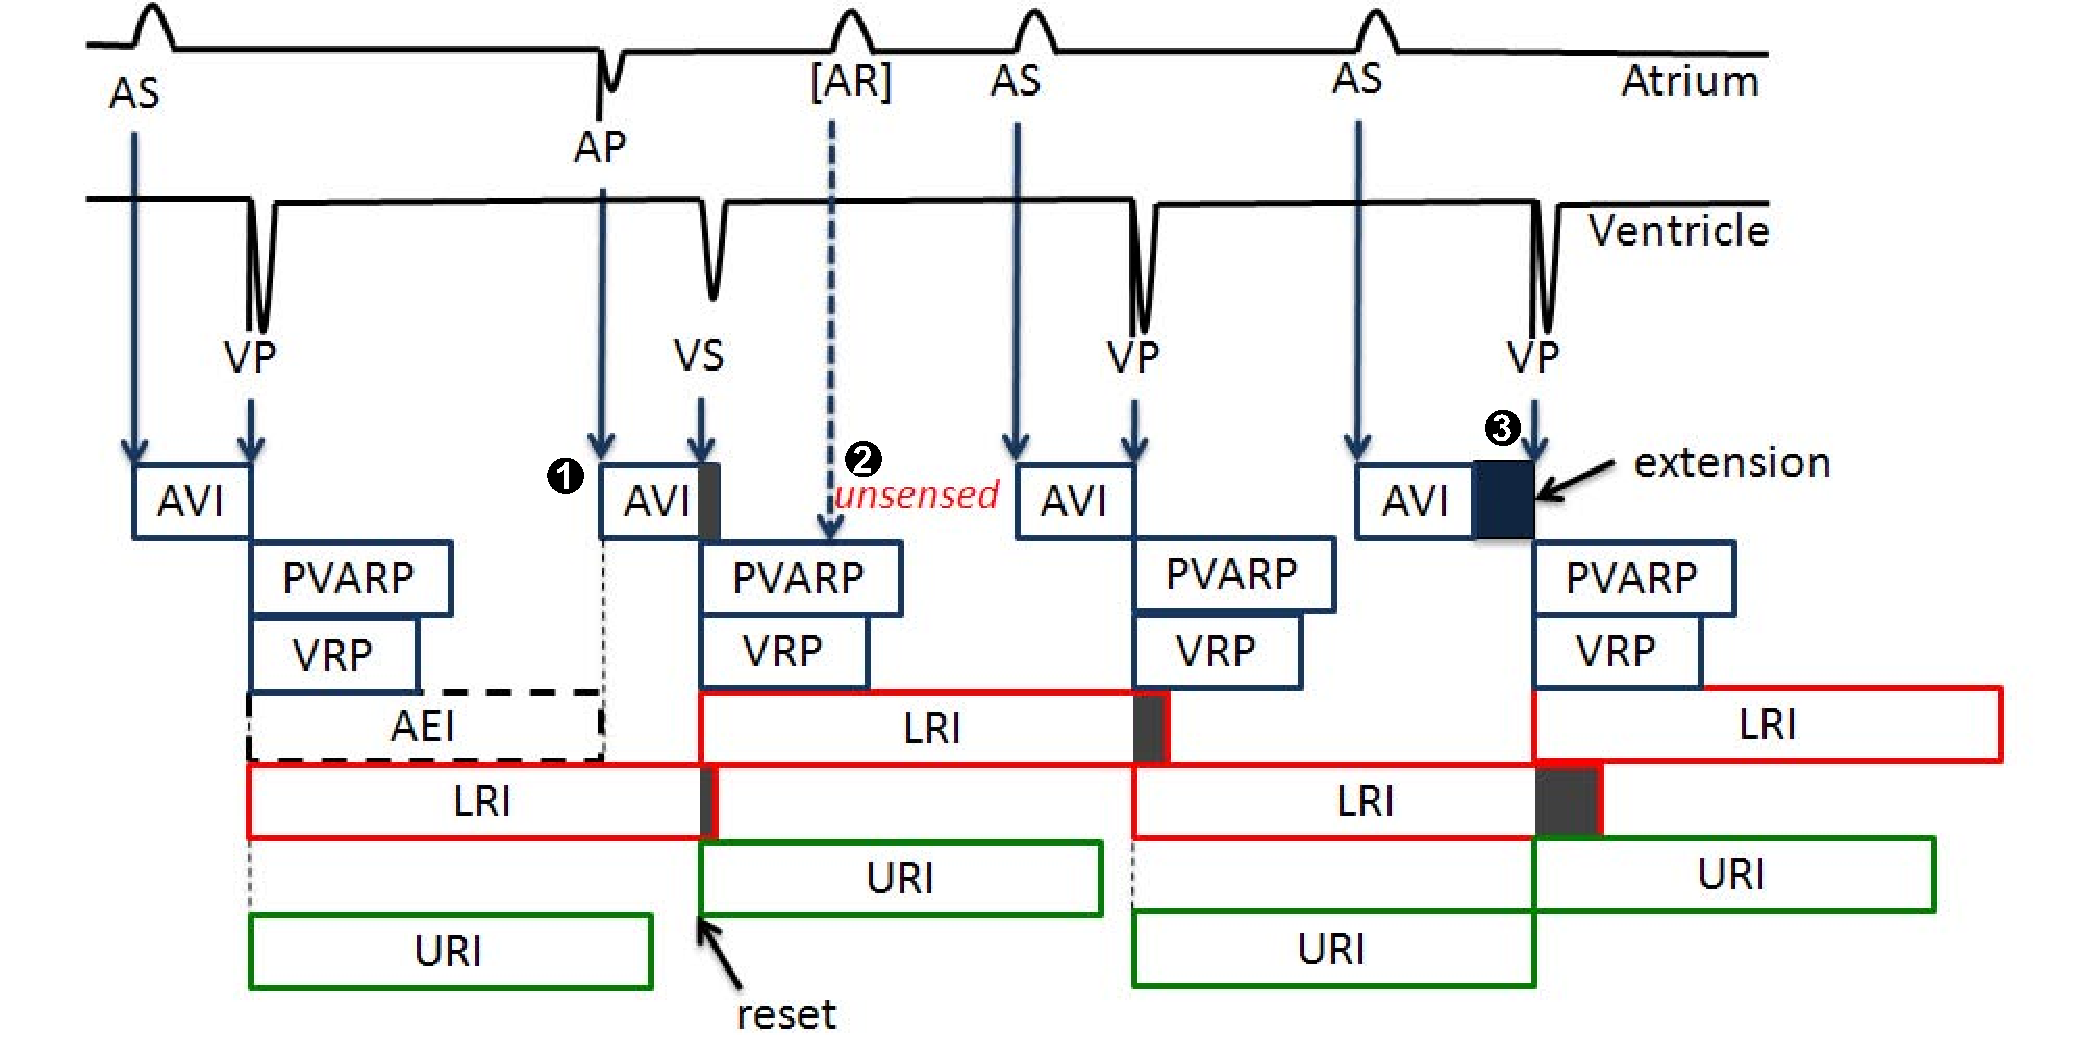
\includegraphics[width=0.85\textwidth]{figs/PM_timers.pdf}
%\vspace{-10pt}
\caption{Basic 5 timing cycles for a dual chamber pacemaker which include the Lower Rate Interval (LRI),  Atrio-Ventricular Interval (AVI), and Upper Rate Interval (URI). Also included are the blanking intervals, Post Ventricular Atrial Refractory Period (PVARP) and Ventricular Refractory Period (VRP), to inhabit action by the pacemaker.}
\label{fig:PMtimers}
%\vspace{-10pt}t

\end{figure} 
A DDD pacemaker has five basic timing cycles triggered by external and internal events, as shown in \figref{PMtimers}. We decomposed our pacemaker model into five components which correspond to the five timers. $P=LRI\| AVI\| URI\| PVARP\| VRP$. These components synchronize with each other using broadcast channels and shared variables (as shown in \figref{PMdesign}). 

\subsection{Lower Rate Interval (LRI)}
%\vspace{-5pt}
The Lower Rate Interval (LRI) component is shown in \figref{PMdesign}(a). This component defines the longest interval allowed between two ventricular events, thus keeping the heart rate above a minimum value. In DDD mode, the LRI interval is divided into a V-A interval (TLRI-TAVI) and a A-V interval (TAVI). The LRI component maintains a maximum V-A delay while the AVI component maintains a maximum A-V delay so together they maintain the maximum V-V delay. In the LRI component, the clock is reset when a ventricular event \textsf{(VS, VP)} is received. If no atrial event has been sensed \textsf{(AS)}, the component will deliver atrial pacing \textsf{(AP)} after TLRI-TAVI. 

%\vspace{-5pt}
\subsection{Atrio-Ventricular Interval (AVI) and Upper Rate Interval (URI)}
%\vspace{-5pt}
The function of the AVI component defines the longest interval between an atrial event and a ventricular event. If there is no ventricular event \textsf{(VS)}  within TAVI after an atrial event \textsf{(AS, AP)}, and the time since the last ventricular event \textsf{(VS, VP)} is longer than TURI, the component will deliver ventricular pacing \textsf{(VP)}. The URI limits the ventricular pacing rate by enforcing a lower bound on the times between consecutive ventricle events. The UPPAAL design of AVI and URI component is shown in \figref{PMdesign}(b) and (c).%The UPPAAL design of AVI component is shown in 

%\vspace{-10pt}
\subsection{Post Ventricular Atrial Refractory Period (PVARP) and Post Ventricular Atrial Blanking (PVAB)}
%\vspace{-5pt}
Ventricular events, especially Ventricular Pace \textsf{(VP)} are sometimes so strong that the atrial lead can sense the activation as well. This signal may be falsely recognized as an atrial event and disrupt normal pacemaker function. This scenario is called crosstalk and was discussed in our previous work (\cite{vhm_embc11}). In order to prevent this undesired behavior, and filter potential noises, there is a blanking period (PVAB) followed by a refractory period (PVARP) for the atrial events after each ventricular event \textsf{(VS, VP)}. Atrial events during PVAB are ignored and atrial events during PVARP trigger \textsf{AR!} events which can be used in some advanced diagnostic algorithms. The UPPAAL design of PVARP component is shown in \figref{PMdesign}(d).

%\vspace{-10pt}
\subsection{Ventricular Refractory Period (VRP)}
%\vspace{-5pt}
The VRP follows each ventricular event \textsf{(VP, VS)} to filter noise and early events in the ventricular channel which could otherwise cause undesired pacemaker behavior. 

\section{Identify Safety Hazards in Implantable Pacemaker}
Implantable pacemakers are designed to treat bradycardia by increasing the heart rate with external pacing. Therefore the heart rate should not only be increased to the minimum physiological need, but also should not be increased beyond physiological need. \figref{risk_req} demonstrates two Fault Tree Analysis (FTA) for these two top level hazards. In the remaining chapter we first specify hazards as properties, and use model checking to evaluate whether these hazards have been mitigated by the pacemaker. Then for one of the mitigation algorithm, we examine the mitigation effectiveness and the residue hazard.
\begin{figure}[!t]
		\centering
		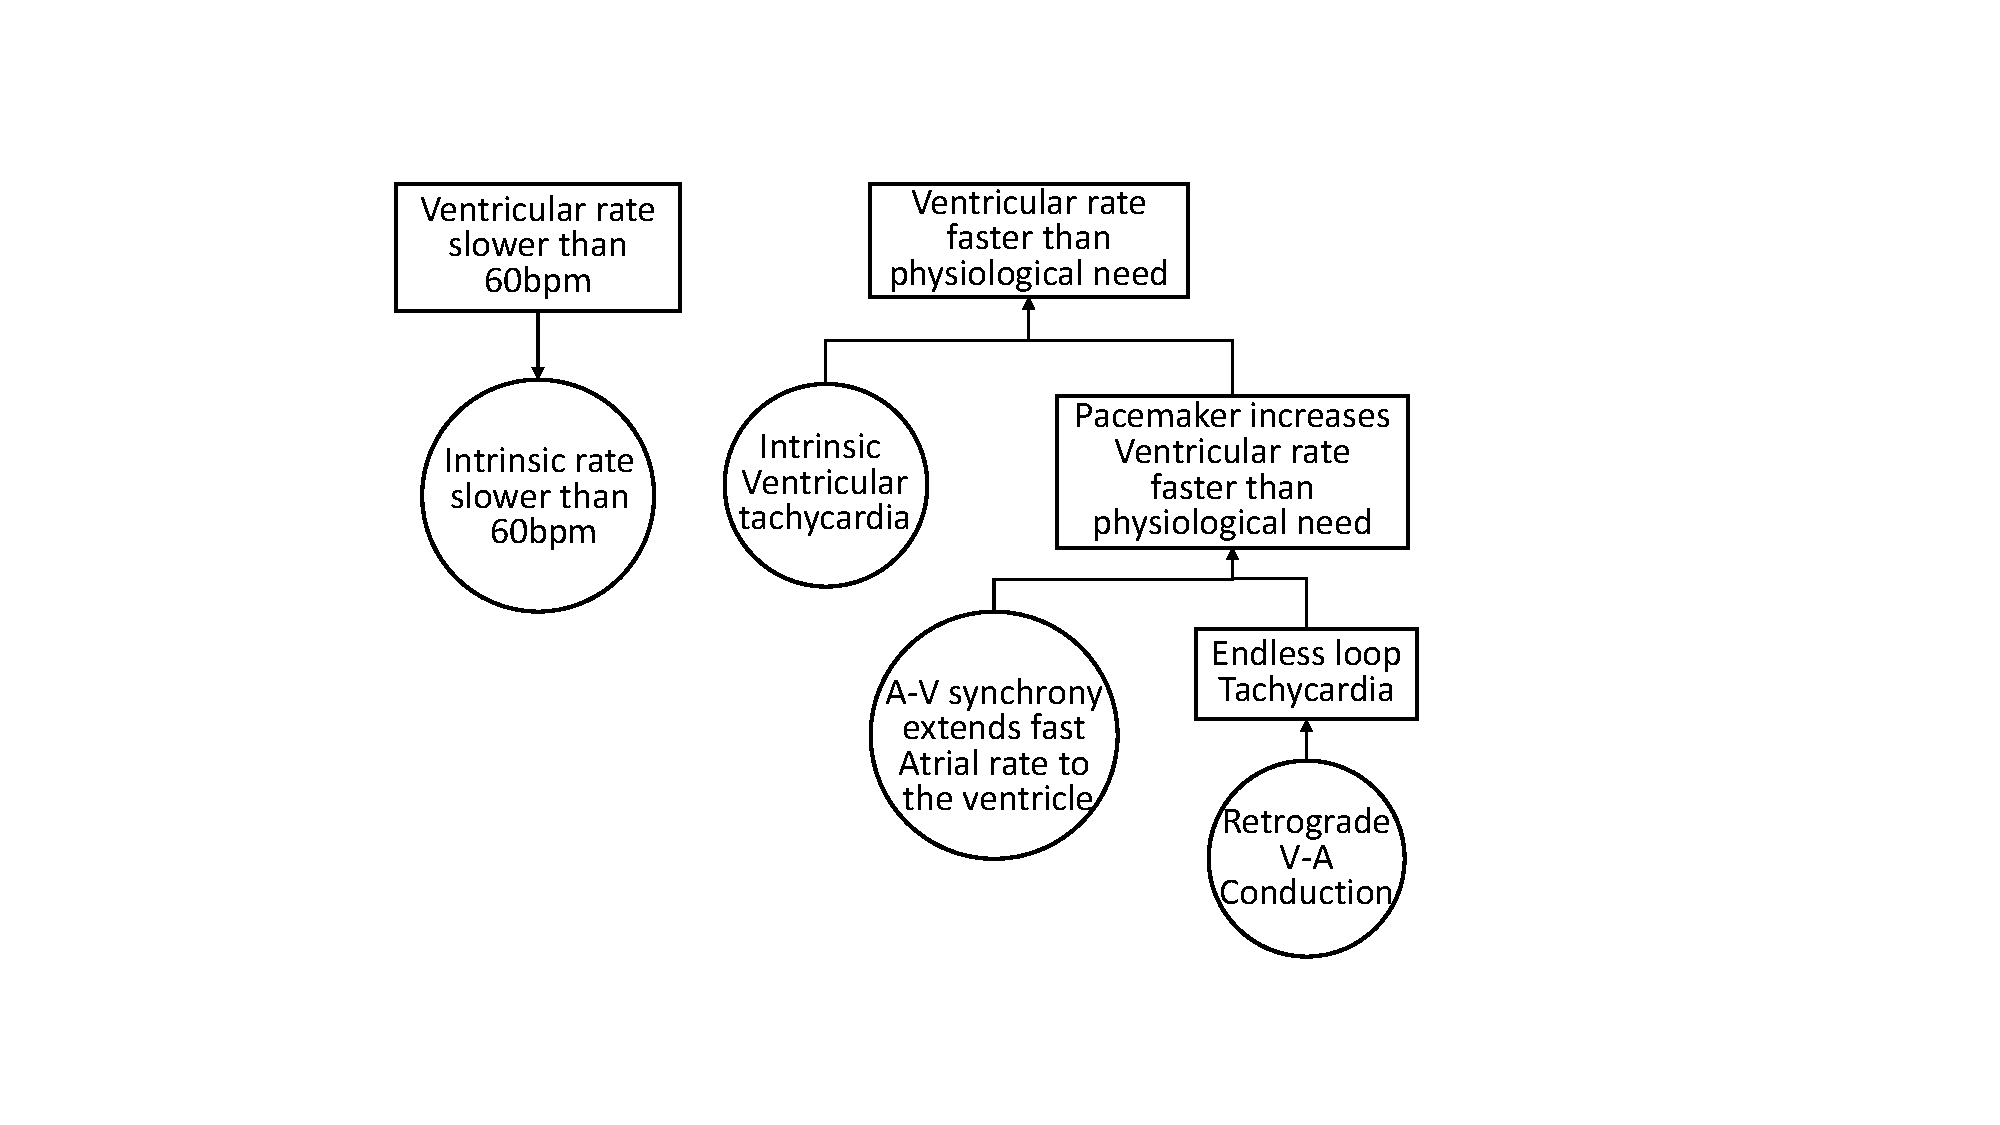
\includegraphics[width=0.8\textwidth]{figs/risk_requirements.pdf}
		\caption{\small Sample Fault Tree Analysis of the physiological conditions leading to the lower rate limit and upper rate limits}
		  %\vspace{-15pt}
		\label{fig:risk_req}
\end{figure}

\section{Known Safety Hazards of Dual Chamber Pacemakers}
In this section we introduce two well-studied safety hazards in a basic dual chamber pacemaker design.
Device manufacturers have developed algorithms to mitigate the hazards.
In the following chapters, I will use model-based techniques to identified these safety hazards in the early design stage, and evaluate the effectiveness of the mitigation algorithms developed by device manufacturers.

\subsection{Endless-Loop Tachycardia}
\begin{figure*}
\centering
%		\vspace{-10pt}
		\subfigure [Virtual circuit formed by the pacemaker and the heart] {
				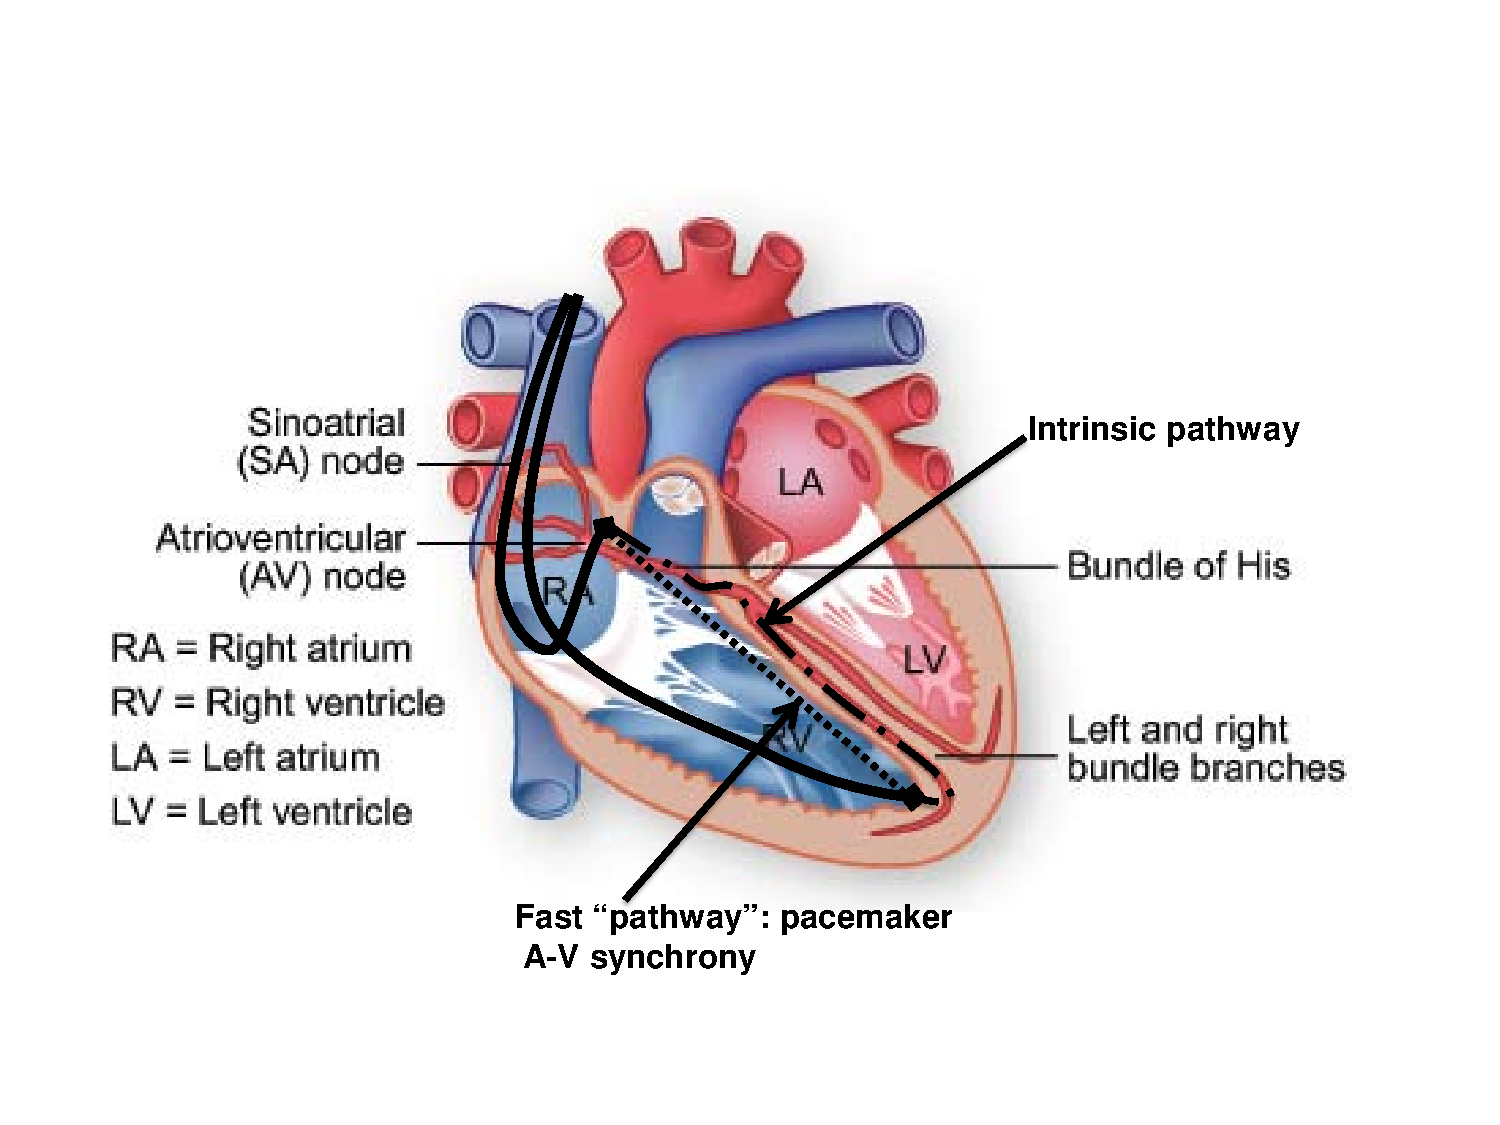
\includegraphics[width=0.4\textwidth]{figs/ELT_str.pdf}
				\label{fig:ELT_demo}
		} 
		\subfigure [Pacemaker trace for ELT initialized by a early ventricular signal]{	
			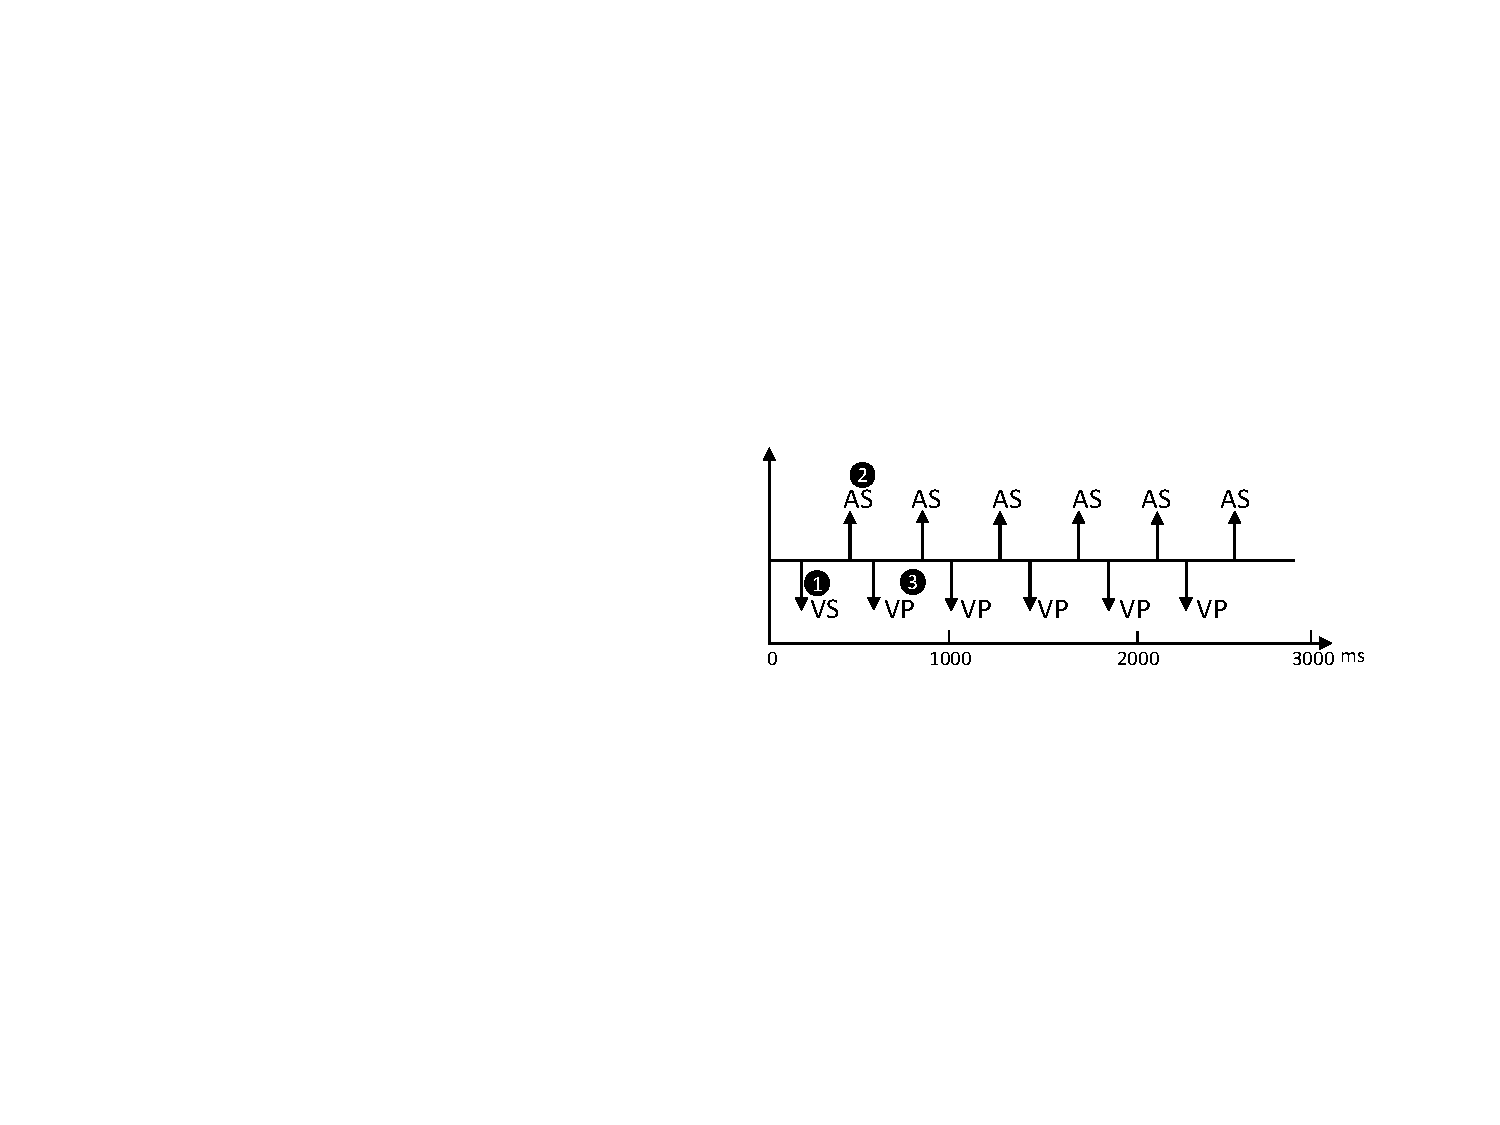
\includegraphics[width=0.4\textwidth]{figs/ELT.pdf}
			\label{fig:ELT}
		}
%		\vspace{-10pt}
	\caption{Endless Loop Tachycardia case study demonstrating the situation when the pacemaker drives the heart into an unsafe state \cite{vhm_iccps11}}
%\vspace{-15pt}
\end{figure*}


The AVI component of a dual-chamber pacemaker introduces a virtual A-V conduction pathway. This forms a timing loop with the intrinsic (physiological) A-V conduction pathway (see \figref{ELT_demo}). A Premature Ventricular Contraction (PVC), i.e. an early extra beat in the ventricles, may trigger another ventricular event (VS) and initiate a V-A conduction through the intrinsic pathway (Marker 1 in \figref{ELT}). The pacemaker registers this signal as an Atrial Sense (AS) (Marker 2 in \figref{ELT}). This event triggers a VP after TAVI, as if the signal conducts through the ``virtual" A-V pathway (Marker 3 in \figref{ELT}). We call it ``virtual" pathway as the ``conduction" delay is fulfilled by a timer in the pacemaker instead of a physical signal propagation along the heart tissue. The VP will trigger another V-A conduction and this VP-AS-VP-AS looping behavior will continue (see \figref{ELT}). The interval between atrial events is TAVI plus the V-A conduction delay, which is normally shorter than the delay between intrinsic heart beats, thus driving the ventricular rate as high as the Upper Rate Limit. During ELT, the heart rate is not only high, but also fixed, which is an unsafe scenario.

\subsection{Atrial Tachycardia Response}

Supraventricular Tachycardia (SVT) is an arrhythmia with an abnormally fast atrial rate. %\figref{SVT} is a series of simulation results for closed-loop interaction between a heart model with SVT and the pacemaker model. The atrial and ventricular channels show electrogram inputs to the pacemaker and the pacemaker channel shows the corresponding events received and generated by the pacemaker software, \cite{vhm_embc11}.
Typically, in a heart without pacemaker, the AV node, which has a long refractory period, can filter most of the fast atrial activations during SVT, thus the ventricular rate remains relatively normal. \figref{SVT_none} demonstrates a pacemaker event trace during SVT, with a pacemaker in ODO mode, which just sensing in both channels. 
As there is no pacing in ODO mode, the heart is in open-loop with the pacemaker. In this particular case, every 3 atrial events (AS) correspond to 1 ventricular event (VS) during SVT. 
As an arrhythmia, SVT is still considered a safe heart condition since the ventricles operate under normal rate and still maintain adequate cardiac output. 

However, in the closed loop case with the DDD pacemaker, the AVI component of a dual chamber pacemaker is equivalent to a virtual pathway in parallel to the intrinsic conduction pathway between the atria and the ventricles. The pacemaker tries to maintain 1:1 A-V conduction and thus increases the ventricular rate inappropriately to match the atrial rate.  This is known as Pacemaker Mediated Tachycardia (PMT) as the heart would have been safe without the pacemaker and its virtual pathway. \figref{SVT_DDD} shows the pacemaker trace of the same SVT case with DDD pacemaker. Although half of the fast atrial events are filtered by the PVARP period ([AR]s), the DDD pacemaker still drives the closed-loop system into 2:1 A-V conduction with faster ventricular rate. Maintaining A-V delay is less important than maintaining an appropriate ventricular rate. The DDD pacemaker violates a higher priority requirement in order to satisfy a lower priority requirement, which is inappropriate.
\begin{figure*}[!t]
\centering
		\subfigure [\small]{			
		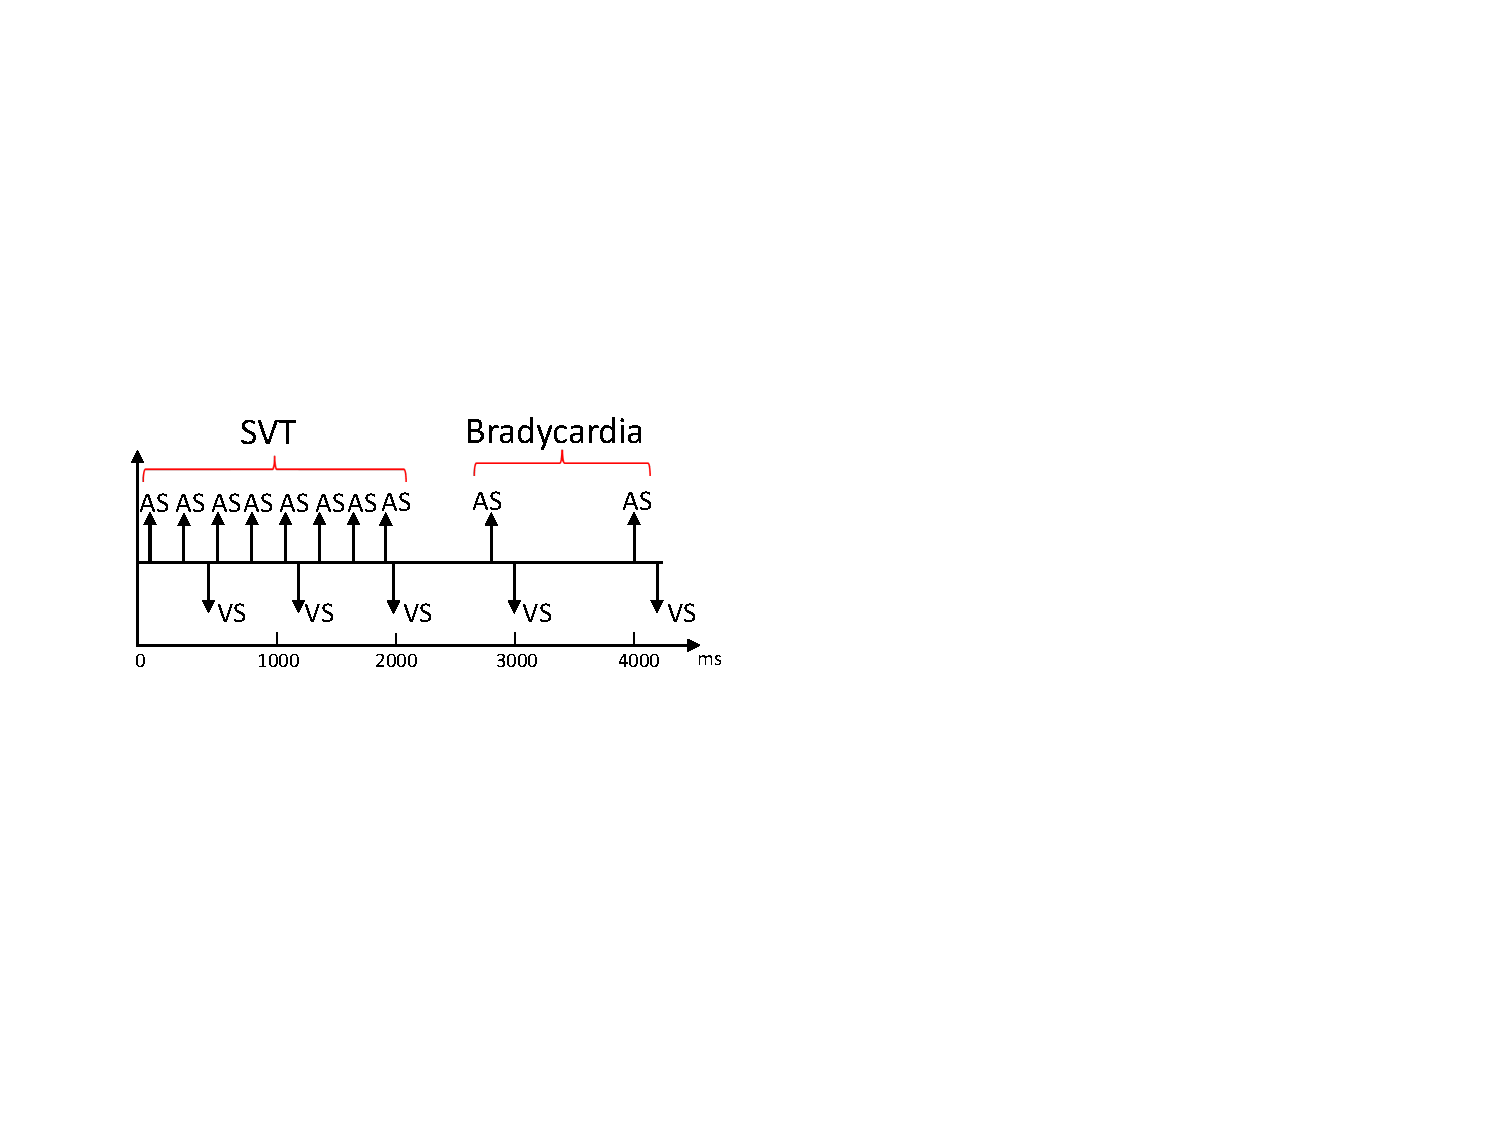
\includegraphics[width=0.5  \textwidth]{figs/SVT_none.pdf}
		\label{fig:SVT_none}
		} 
%	\hspace{.1in}%
\vspace{-10pt}
		
		\subfigure [\small] 
		{
		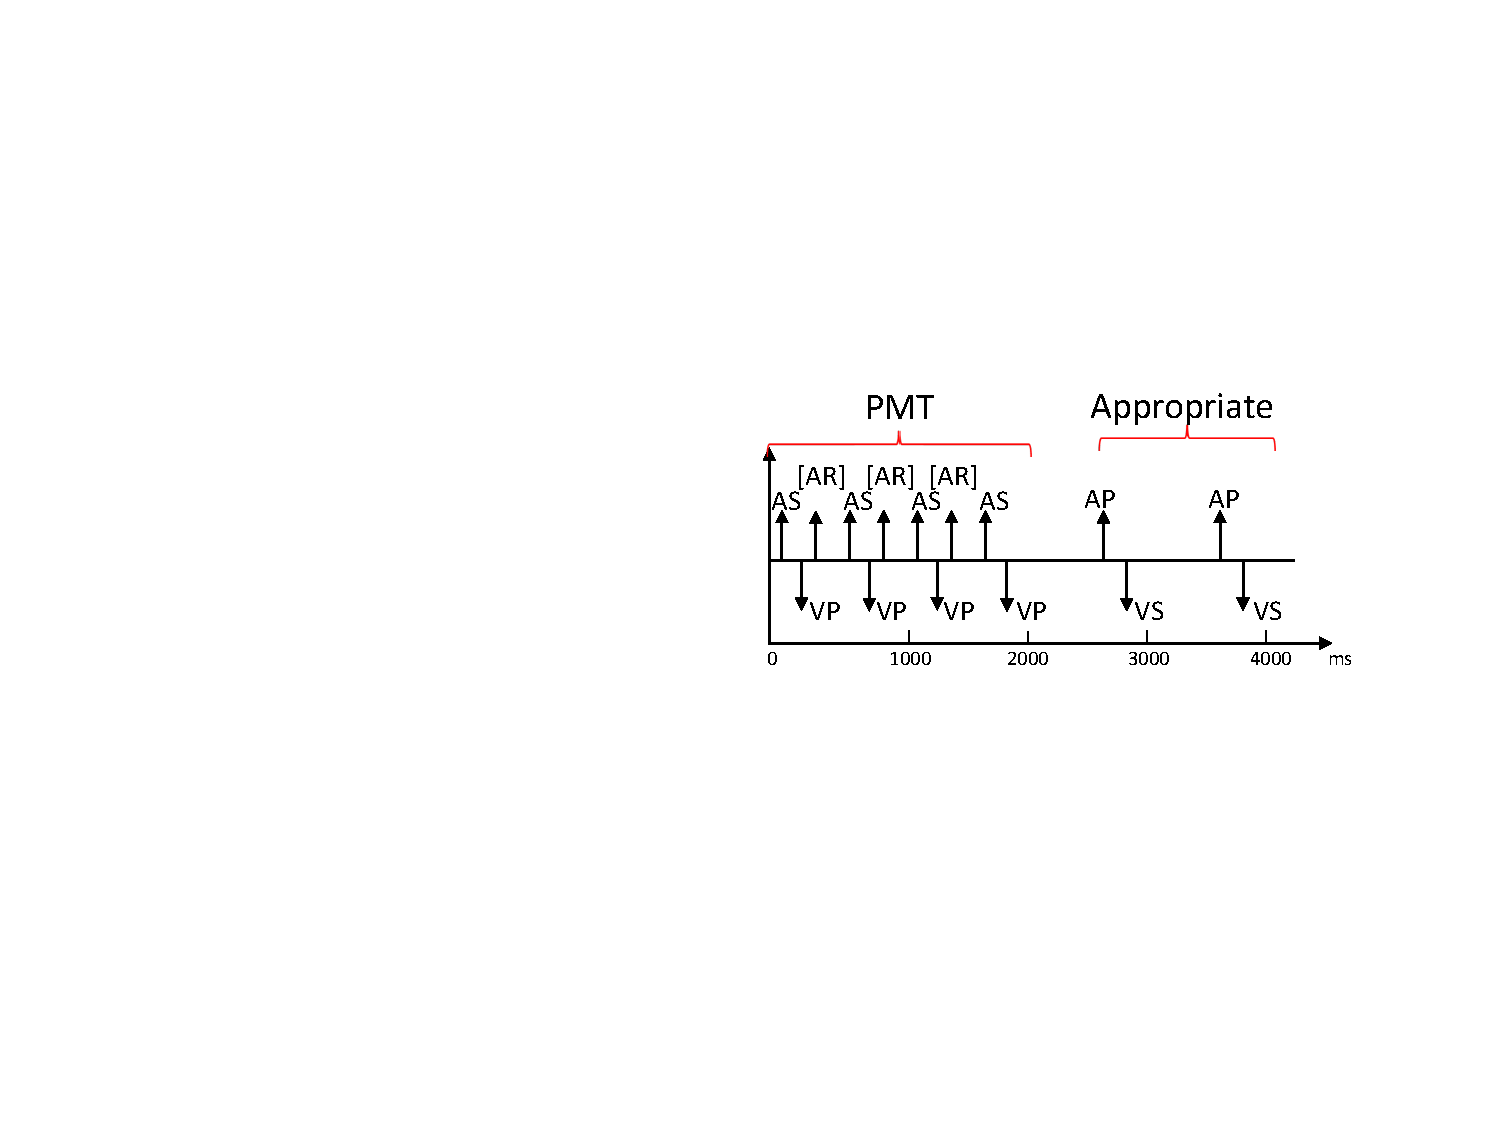
\includegraphics[width=0.5\textwidth]{figs/SVT_DDD.pdf}
		\label{fig:SVT_DDD}
		} 
\vspace{-5pt}
\caption{\small Benign open loop case: SVT without a pacemaker or with a pacemaker in sense-only mode (ODO) (b) Dangerous closed-loop-case SVT with DDD pacemaker which tries to match the fast atrial rate with a corresponding (and dangerous) fast ventricular rate.}
\vspace{-10pt}
\end{figure*} 

\section{Discussion}
Implantable cardiac devices such as implantable pacemakers are typical autonomous medical devices.
Although the functionality is relatively simple, pacemakers illustrate the three challenges discussed in the introduction very well.
In the following chapters, I will demonstrate the use of different model-based techniques to provide safety and efficacy confidence to the pacemaker design.


